\documentclass[aspectratio=1610, xcolor=dvipsnames]{packages/beamer}

\setbeamertemplate{navigation symbols}{}


%\input{smile_styles}
\usepackage[nolist,nohyperlinks]{acronym}


\usetheme{Madrid}
\useinnertheme{circles}
\useoutertheme{infolines}
\usefonttheme{serif}
\usepackage{etoolbox}
\definecolor{UBMaroon}{rgb}{0.3, 0.0, 0.0} % UBC Blue (primary)
\definecolor{UBBlackPurple}{rgb}{0.1, 0.07, 0.12} % UBC Blue (primary)
\usecolortheme[named=UBBlackPurple]{structure}

% \usepackage[cache=false]{minted}
\usepackage{amsthm}
\usepackage{amsmath}
\usepackage{amssymb,mathtools}
\usepackage[longend]{algorithm2e}
\usepackage{textgreek}
\usepackage{tcolorbox}
\usepackage{listings}
\usepackage{textcomp}
\usepackage[style=authortitle,backend=biber]{biblatex}
\usepackage{caption}
\usepackage{subcaption}
\usepackage{color}
\usepackage{graphicx}
\usepackage{ifthen}
\usepackage{xparse}
%\usepackage{enumitem}
%\setlist[enumerate,1]{label={(\arabic*)}}

\newcommand{\displayTOC}{\begin{frame}\frametitle{Agenda} \tableofcontents[currentsection, subsectionstyle=show/show/hide]\end{frame}}
\newcommand{\argmax}{\operatornamewithlimits{argmax}}
\newcommand{\jointS}{\bar{\mathbf{S}}}
\newcommand{\jointA}{\bar{\mathbf{A}}}
\newcommand{\joints}{\bar{s}}
\newcommand{\jointa}{\bar{a}}
\newcommand{\add}{\textcolor{red}}



\NewDocumentCommand{\cond}{ O{} O{}}{
 \ifthenelse { \equal{#1}{} }
        {\ifthenelse { \equal{#2}{}}
            {\mathcal{C}}               % [][]
            {\mathcal{C}_{\pi_{#2}}}    % [][#2]
        }   % if #1 == blank
        {\ifthenelse { \equal{#2}{} }
            {\mathcal{C}^{\hat{\pi}_{#1}}}  %[#1][]
            {\mathcal{C}^{\hat{\pi}_{#1}}_{\pi_{#2}}} %[#1][#2]
        }
}
\DeclareMathOperator{\CPT}{\mathbb{C}}
\DeclareMathOperator{\Expect}{\mathbb{E}}
\DeclareMathOperator{\Ind}{\mathbb{1}}

\DeclareMathOperator{\forall}{\;\;\forall\;}
% \newcommand{\joint}[1]{\bar{#1}}
\newcommand{\joint}[1]{#1}



\addbibresource{packages/references.bib}
\hypersetup{
        unicode=true,
        linkcolor=blue,
        anchorcolor=blue,
        citecolor=green,
        filecolor=black,
        urlcolor=blue
    }

%#########################################################
%#########################################################
%#########################################################
\title{Fall 2022 - Winter Break Update}\author{Mason Smith}\date\today
\begin{document}\begin{frame}[plain]\titlepage\end{frame}


\begin{acronym}
    \acro{RL}{reinforcement learning}
    \acro{QRE}{Quantal Response Equilibrium}
     \acro{ToM}{Theory of Mind}
     \acro{AUIC}{area under the indifference curve}
     \acro{CPT}{cumulative prospect theory}
\end{acronym}




%%%%%%%%%%%%%%%%%%%%%%%%%%%%%%%%%%%%%%%%%%%%%%%%%%%%%%%%%%%
%%%%%%%%%%%%%%%%%%%%%%%%%%%%%%%%%%%%%%%%%%%%%%%%%%%%%%%%%%%
%%%%%%%%%%%%%%%%%%%%%%%%%%%%%%%%%%%%%%%%%%%%%%%%%%%%%%%%%%%
\section{Introduction} \displayTOC

\begin{frame}{Fall 2022 Discoveries:}
    \begin{itemize}
        \item Simulation of assuming bias policies revealed trivial effects
        \begin{itemize}
            \item Mainly, performance would be \textit{ all or nothing} for training averse vs seeking conditions policies
            \item Same \textit{all or nothing} behavior was shown when switching assumptions
        \end{itemize}
        \item Discovered that this is primarily a product of game design and training approach
        \item My problem has the past few weeks has been slightly tedious in tweaking highly sensitive hyper parameters
        and game designs s.t.performance in the aforementioned scenarios is a continuous spectrum able to be compared.
    \end{itemize}
\end{frame}

\begin{frame}{Introduction}
    Current Work:
    \begin{itemize}
        \item Improving game design to allow for consistent training
        \item Training stable CPT value functions that represent biased policies
        \item Redesigning world and retraining to ensure non-trivial differences
        \begin{itemize}
            \item Do not complete with unrelated or identical strategies
            \item Want to achieve the objective (catch the target) with semi-similar success rate in different ways (trajectories)
        \end{itemize}
        \item Testing effects of assuming different biases for H in simulation
    \end{itemize}
    Challenges: \begin{itemize}
        \item Was struggling with getting stuck in local optima due to sparse gains (catch at end of game) and frequent penalties (throughout the game)

        \item There is a sensitive and fine balance for the following hyper-parameters that induce interesting policies to contrast:
        \begin{itemize}
            \item Admissible bounds for risk-sensitivity
            \item World design and initial conditions
            \item Learning hyper-parameters
        \end{itemize}
    \end{itemize}

\end{frame}

%#########################################################
%#########################################################
%#########################################################
\section{Game Design Update} \displayTOC

\subsection{Issues with Current Game}
\begin{frame}{Issues with Current Game}
    \begin{itemize}
        \item Algorithm gets stuck in local optima due to
        \begin{itemize}
            \item sparse gains (catch at end of game)
            \item frequent penalties (throughout the game)
            \item Strong encouragement to wait out the rest of the game once a penalty is received (do not chase target anymore)
        \end{itemize}

        \item Different worlds induced differences in bias policies that were either
        \begin{itemize}
            \item too strong
            \begin{itemize}
                \item risk-averse had 0\% catch rate while risk-seeking had 100\% catch rate
                \item When switching to incorrect assumption $\rightarrow 0$\%  catch rate
                \item impossible to evaluate coordination strategies were incompatible or had same outcome
            \end{itemize}
            \item too weak
            \begin{itemize}
                \item both policies either had near 100\% or both had 0\% performance
                \item solution is so obvious that CPT does not change it
                \item again produced trivial result due similarity between strategies
            \end{itemize}
        \end{itemize}
    \end{itemize}
\end{frame}


\subsection{Update Goals}
\begin{frame}{Update Goals}
\begin{itemize}
        \item Produce two policies (averse and seeking) that
        \begin{itemize}
            \item produce compatible strategies that achieve the objective $p(success) - \epsilon > 0$ when paired
            \item produce sufficiently unique joint-behavior when mis-matching policies compared to matching policies
            \item produce sufficiently similar performance between matched-averse and matched-seeking policies s.t. comparison between is valid
        \end{itemize}
        \item Modify
        \begin{itemize}
             \item world configurations (initial positions and penalty positions)
             \item global game rules and game hyper-parameters
        \end{itemize}
    \end{itemize}
\end{frame}

\subsection{List of Updates}
\begin{frame}{List of Updates}
    \begin{itemize}
        \item Redesigned world initial states and penalty locations
        \begin{itemize}
            \item remove low-effect and difficult to train worlds
        \end{itemize}
        \item Reward for catching target $r(catch)= 20 \rightarrow 25$
        \begin{itemize}
            \item increasing window to receive positive reward $\sum r_{t} >0$ after penalties and $-1$ turn reward are added
        \end{itemize}
        \item Reward is now delivered as a single cumulative reward $r_\zeta$ at the end of the game
        \begin{itemize}
            \item previously provided reward at every time-step $r_{t}$
            \item helps avoid getting stuck local optima since intermediate rewards were only penalties
            \item evaluates reward on a trajectory-scope $r_\zeta(\mathbf{s}_T,\mathbf{a}_T)$
            \item instead of action-scope $r_{t}(s_t,a_t)$ where $r_\zeta = \sum_{t\in T} \; r_t$
            \item apply eligibility traces ($TD(\lambda)$) to account for increased sparsity
        \end{itemize}
        \item Reward is now non-negative
        \begin{itemize}
            \item the cumulative reward at the end of the game is $r_\zeta = max(r_\zeta,0)$
            \item new objective: maximize your reward \textbf{upon catching the target}
            \item doing really bad and not catching the stag are now equivalent
            \item eliminates trivial policy of avoiding rewards by never moving (especially relevant in averse-conditions)
        \end{itemize}
    \end{itemize}
\end{frame}

\subsection{Updated World Designs}
\begin{frame}{Updated Worlds}
    \begin{figure}
        \centering
        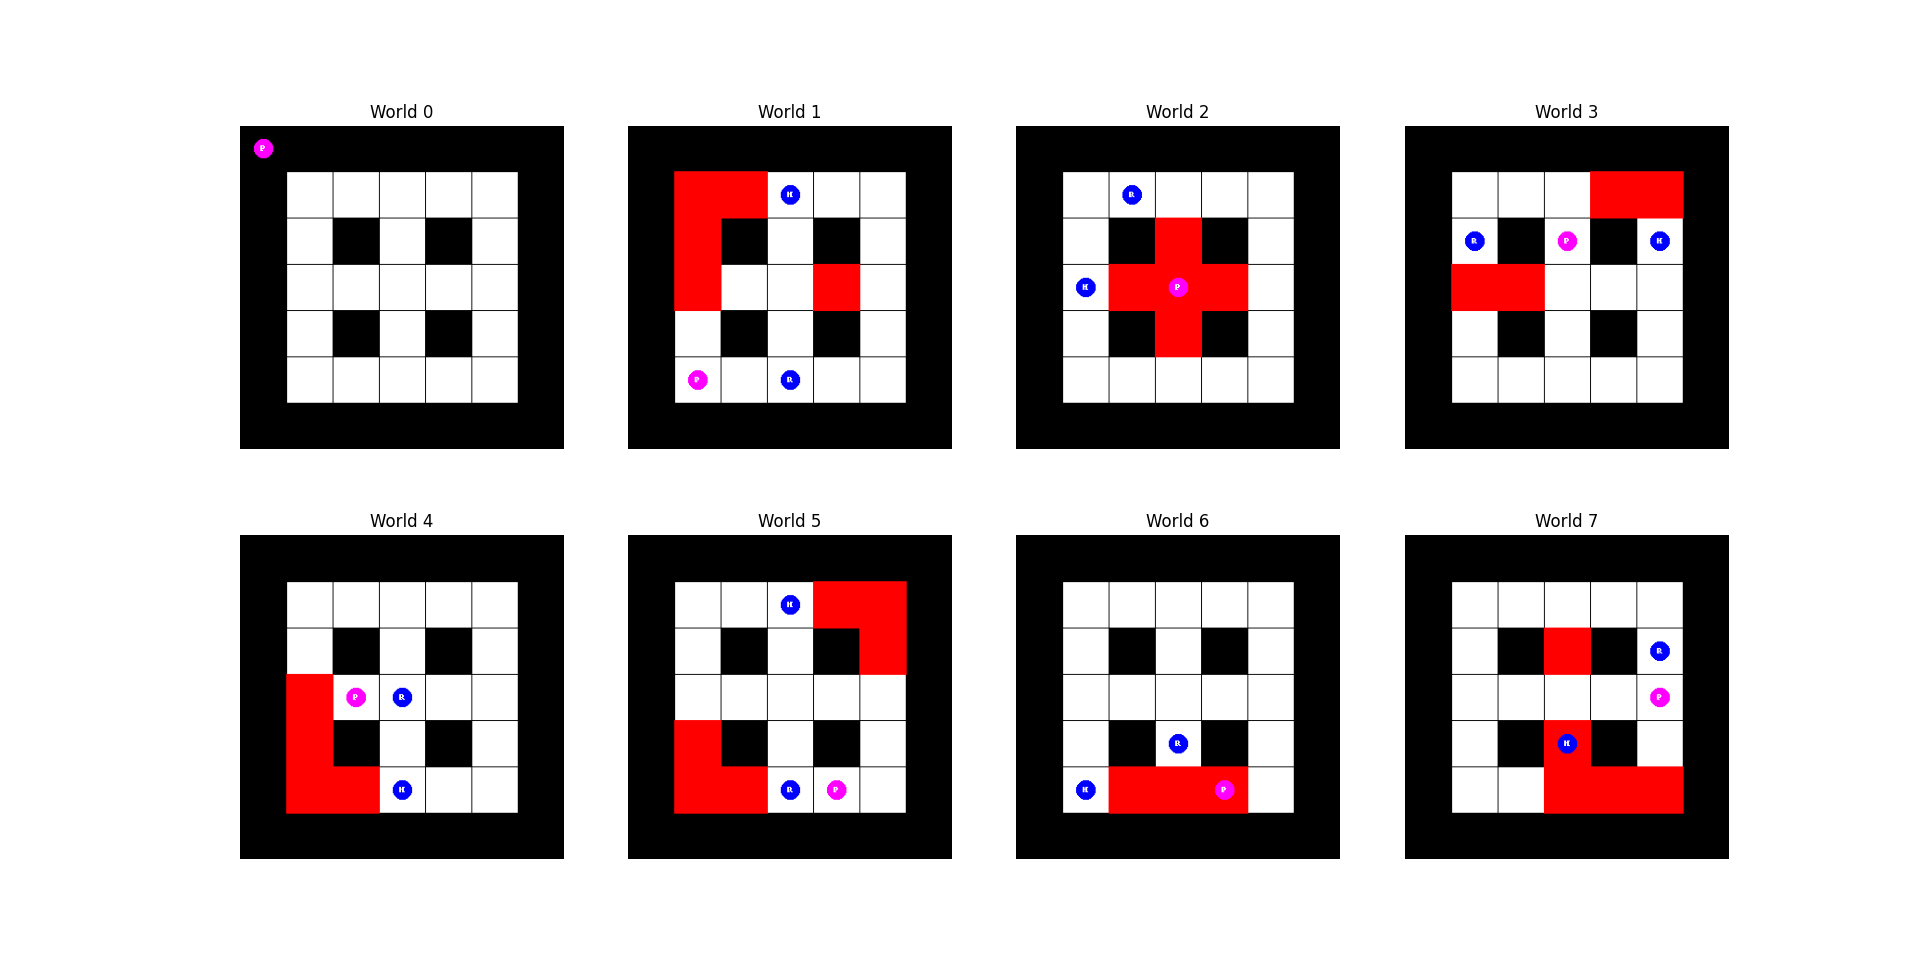
\includegraphics[width=0.95\textwidth]{../results/Fig_Worlds}
        \caption{Updated World Designs}
        \label{fig:Worlds}
    \end{figure}

\end{frame}
%#########################################################
%#########################################################
%#########################################################
\section{Training Policies} \displayTOC



\subsection{Training Setup} \begin{frame}{Training Setup}
    \begin{itemize}
        \item Implemented a independent joint-Q learning algorithm with directed exploration and \ac{ToM}
        \item \Ac{QRE} used as the equilibrium condition to solve games at every stage (\ac{ToM})
        \item Trained 3x policies $\pi$ trained during self-play:
        \begin{itemize}
            \item baseline/optimal ($\pi_{0}$)
            \item risk-averse ($\pi_{A}$)
            \item risk-seeking ($\pi_{S}$)
        \end{itemize}
        \item Baseline policy $\pi_{0}$ was used as prior for biased policies $\pi_{A}$ and $\pi_{S}$ trained with \ac{CPT} agents
        \item Sophistication (level of recursion) was set to 3 in the \ac{QRE}
    \end{itemize}
\end{frame}

\subsection{Algorithm}

\begin{frame}{Notation}
\begin{itemize}
    \item  $\times$ denotes the Cartesian product and $(\cdot)$ an unfilled index/value
    \item ego agent denoted by subscript $(\cdot)_k$ where $(\cdot)_{-k}$ represents the partner and $k,-k \in K$
    \item joint state $\joint{s} \in \joint{S}$ where $ \joint{S} = S_{k} \times S_{-k}$
    \item joint action $\joint{a} \in \joint{A}$ where $ \joint{A} = A_{k} \times A_{-k}$
    \begin{itemize}
        \item $\joint{a}$ may be written as $\joint{a}=\{a_k,a_{-k}\}$ for clarity
        \item alternativley, $\joint{a}$ expressed as policies $\joint{a}=\{\pi_{k}(\joint(s)),\pi_{-k}(\joint(s))\}$
    \end{itemize}
    \item ego stage reward $r_t$
    \item let $e_k(\joint{s},\joint{a})$ denote an eligibility trace keeping track of state visitations within an episode that decays by $\lambda$ each step
    \item let $\CPT[(\cdot)]$ denote the expected value of rewards given true rewards and a CPT transformation
    \item let $\mathcal{P}_{CPT} = \{b,l,\gamma^{+},\gamma^{-},\delta^{+},\delta^{-}\}$ denote a set of CPT model parameters
\end{itemize}

\end{frame}

\begin{frame}{Notation}
\begin{itemize}
    \item a policy $\pi_k$
    \begin{itemize}
        \item always denotes choosing ego action $a_k$ in state $\joint{s}$
        \item $a_k$ sampled from \textit{joint state-joint action} values $Q_k(\joint{s},\joint{a})$
        \item requires inferring partner $-k$ policy $\hat{\pi}_{-k}$
        \item $Q_k(\joint{s},\joint{a})$ is reduced to \textit{joint state-ego action} values $Q_k(\joint{s},a_k)$ by
        \begin{itemize}
            \item conditioning on $\hat{\pi}_{-k}$
            \item s.t. $Q_k(\joint{s},a_k) = \mathbb{E}\big[Q_k(\joint{s},\joint{a} | \joint{a} = \{a_k,a_{-k}=\hat{\pi}_{-k}(\joint{s})\})\big]\; \forall a_k \in A_k$
        \end{itemize}
        \item $a_k$ is drawn from $Q_k(\joint{s},a_k)$ using a nominal Boltzmann dist. \footnote{nominal implies that rationality =1}
        \item for brevity this reduction will be implied and we will write
        $Q_k(\joint{s},\{a_k,\hat{\pi}_{-k}(\joint{s})\})$ to denote the full expression
        $\mathbb{E}\big[Q_k(\joint{s},\joint{a} | \joint{a} = \{a_k,a_{-k}=\hat{\pi}_{-k}(\joint{s})\})\big]\; \forall a_k \in A_k$
    \end{itemize}
    \item let a hat indicate that a parameter is inferred/estimated $\hat{\cdot}$
    \item let a tilde indicate that a parameter\footnote{namely reward and value} was transformed, by CPT,
    into the  perceived values of those parameters $\tilde{\cdot}$
\end{itemize}

\end{frame}

\begin{frame}{Algorithm}
%    {\small
    \begin{tcolorbox}[fonttitle=\bfseries, title=Joint-$TD(\lambda)$ ]
    \begin{algorithm}[H]
%        \algsetup{linenosize=\tiny}
        \tiny
        \scriptsize
        Initialize $Q_k(\joint{s},\joint{a})$ arbitrarily for all $\joint{s},\joint{a}$ \\
        \ForEach{episode}{
            Initialize $\joint{s}$ and $e_k(\joint{s},\joint{a}) = \mathbf{0}$  \\
            \ForEach{step of episode}{
                $a_k \leftarrow$ ego action given by $\pi_{k}(\joint{s} | \hat{\pi}_{-k}(\joint{s}))$ \\
                Take action $a_k$, observe joint action $\joint{a}$, rewards $r_{k}$, and next state $\joint{s}'$ \\
            % $\delta \leftarrow r+\gamma Q_k(\joint{s}',\joint{a}') - Q_k(\joint{s},\joint{a}) $ \\
            % $\delta \leftarrow r+\gamma\max_{a'_k} \mathbb{E}\{Q_k(\joint{s}',\{a'_k,a'_{-k}\} | a'_{-k} = \hat{\pi}_{-k}(\joint{s}'))\}  - Q_k(\joint{s},\joint{a}) $ \\
            % $\delta \leftarrow r_k+\gamma\max_{a'_k} \mathbb{E}\big[Q_k(\joint{s}',\joint{a}' | \joint{a}' = \{a'_k,\hat{\pi}_{-k}(\joint{s}')\})\big]  - Q_k(\joint{s},\joint{a}) $ \\
                $\delta \leftarrow r_k+\gamma\max_{a'_k} Q_k(\joint{s}',\{a'_k,\hat{\pi}_{-k}(\joint{s}')\})  - Q_k(\joint{s},\joint{a}) $ \\
                $e_k(\joint{s},\joint{a}) \leftarrow e_k(\joint{s},\joint{a}) +1$ \\
                \ForEach{\joint{s} \times \joint{a}}{
                    $ Q_k(\joint{s},\joint{a}) \leftarrow  Q_k(\joint{s},\joint{a}) + \alpha \delta  e_k(\joint{s},\joint{a})$\\
                    $e_k(\joint{s},\joint{a}) \leftarrow \gamma \lambda e_k(\joint{s},\joint{a}) $ \\
                }
                $\joint{s},\joint{a} \leftarrow \joint{s}',\joint{a}'$ \\
                Until $\joint{s}$ is terminal \;
            }
        }
        \label{alg:algorithm}
    \end{algorithm}
    \end{tcolorbox}

%    }
\end{frame}






\begin{frame}{Area Under the Indifference Curve (AUIC)}
        \ac{AUIC} is an expression of preference for accepting or rejecting a gamble over actions with certain outcomes in terms of probabilities $p(accept)$

        \begin{itemize}
            \item \ac{AUIC} is evaluated over space of feasible rewards $\mathbf{R}$ in the game
            \item Define binomial-choices ($a_1,a_2$)
            \begin{itemize}
                \item with outcomes sampled from $\mathbf{R}$ s.t. $\mathbf{R}_{1},\mathbf{R}_{2} = \mathbf{R}$
            \end{itemize}
            \item The outcomes of each choice are then:
            \begin{itemize}
                \item $a_{1}$ containing one certain outcome
                \begin{itemize}
                    \item  with possible rewards $\mathbf{R}_{1} = \{r_1 -0.5*r_{\rho} \;\forall\; r_1 \in \mathbf{R}_{1}\}$
                \end{itemize}
                \item $a_{2}$ containing two uncertain outcomes (with/without penalty $r_\rho$)
                \begin{itemize}
                    \item with possible rewards $\mathbf{R}_{2} = \{[r_2,(r_2 -r_\rho)] \;\forall\; r_2 \in\mathbf{R}_2\}$
                    \item with probabilities $p = [(1-p_{\rho}),p_{\rho}]$ for each outcome occurring
                \end{itemize}
            \end{itemize}


        \end{itemize}
\end{frame}


\begin{frame}{Area Under the Indifference Curve (AUIC)}
    \begin{itemize}
        \item \textit{Indifference Curve}:\footnote{white line in the following figures}
        \begin{itemize}
            \item a continuous curve through the 2D reward space ($\mathbf{R}_{1} \times \mathbf{R}_{2}$)
            \item occurs when no preference is expressed s.t. $p(accept) = 1-p(accept)$
        \end{itemize}
        \item $p(accept)=p(a_2)$ then implies risk-sensitivity where
        \begin{itemize}
            \item An optimal agent expresses no preference\footnote{is indifferent when presented choices} given $r_1=r_2 \;\forall\; r_1,r_2 \in \mathbf{R}$
            \item Preferences become more complex as we apply CPT $\mathbb{C}[(\cdot)]$
        \end{itemize}
        \item \ac{AUIC}\footnote{also be described as a preference anomaly but a modified-AUIC is more consistent with the literature} will be calculated as follows:
        \begin{itemize}
            \item Expresses the cumulative (mean) probability of $p(accept)$ across a symmetrical space of rewards transformed by CPT
            \item Centered around $0$ for legibility s.t. AUIC$\in (-0.5,0.5)$
            \item \ac{AUIC} $=\frac{1}{|\mathbf{R}_1 \times \mathbf{R}_2|} \sum_{r_1,r_2\in \mathbf{R}_{1},\mathbf{R}_{2}}  p(accept | \mathbb{C}[r_1,r_2]) - 0.5$
        \end{itemize}
    \end{itemize}
\end{frame}

\begin{frame}{Interpretting AUIC}

    \begin{itemize}%[leftmargin=0.2\textwidth]
%        \setlength{\leftmargini}{0.2\textwidth}]
%        \addtolength{\itemindent}{0.2\textwidth}
%        \setlength{\itemindent}{0.2\textwidth}
        \item $\text{\ac{AUIC}} < p_{\epsilon} $: the agent cumulatively prefers rejecting the gamble and is risk-averse
        \item $\text{\ac{AUIC}} > p_{\epsilon}$: the agent cumulatively prefers accepting the gamble and is risk-seeking
        \item $|\text{\ac{AUIC}}| < p_{\epsilon}$: the agent agent has week cumulative preferences and is risk-insensitive
        \item $\text{\ac{AUIC}} = 0$: the agent has no cumulative preferences and is optimal
    \end{itemize}
    \begin{itemize}
        \item where $p_{\epsilon}=0.1$ is a threshold defining what we consider risk-sensitive
    \end{itemize}
\end{frame}

\begin{frame}{Area Under the Indifference Curve (AUIC)}
     \begin{figure}
        \centering
        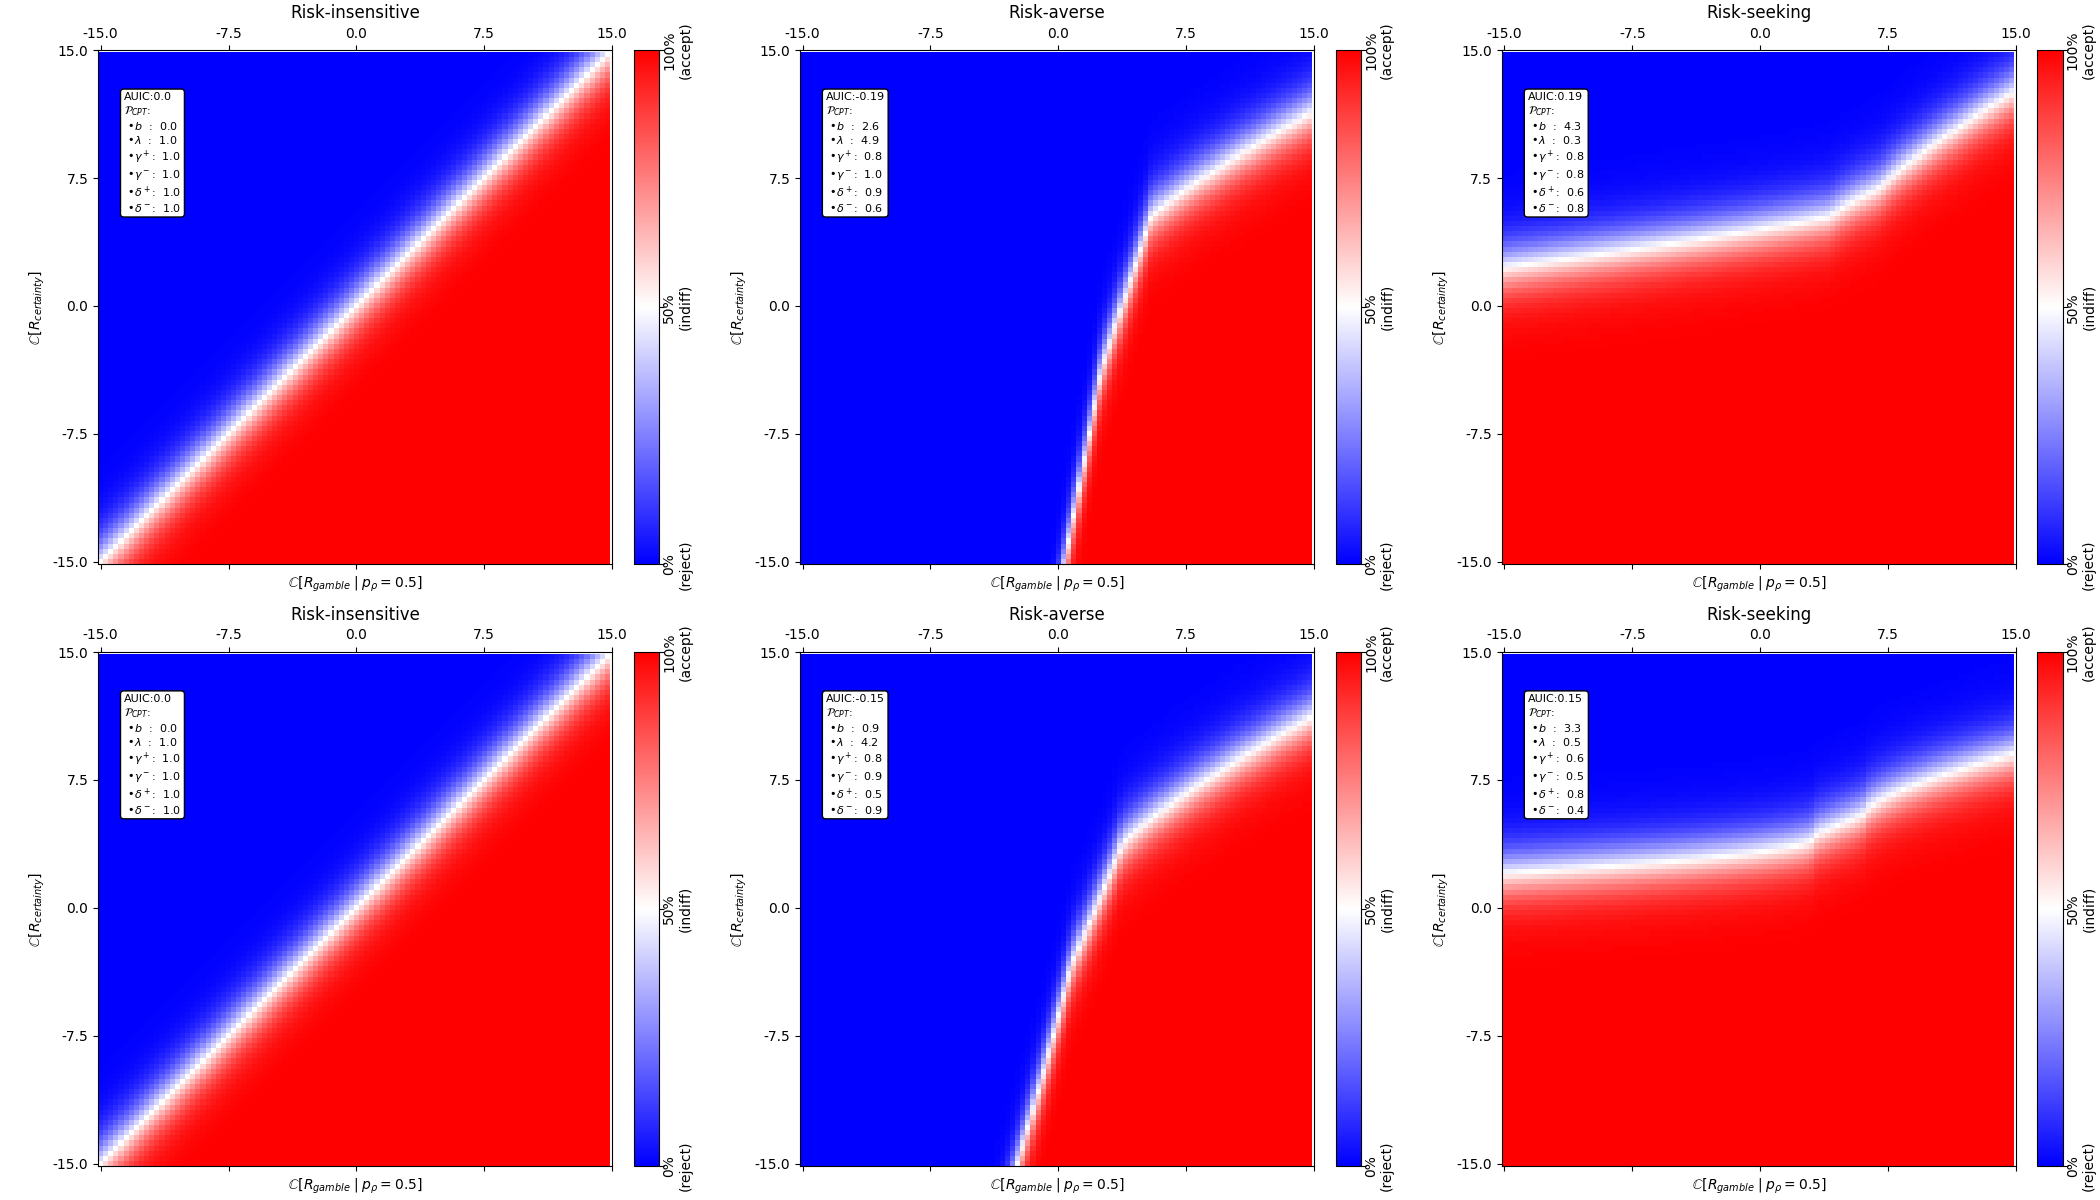
\includegraphics[width=0.95\textwidth]{../results/Fig_AUIC}
        \caption{AUIC Samples}
        \label{fig:AUIC}
    \end{figure}

\end{frame}


\subsection{Creating Biased Policies}\begin{frame}{Creating Biased Policies}
    \begin{itemize}
        \item \Ac{CPT} parameters $\mathcal{P}_{CPT}$ were stochastically perturbed while training biased policies
        \begin{itemize}
            \item $\mathcal{P}_{CPT}$ were sampled in batches every 200 episodes
            \item $\mathcal{P}_{CPT}$ were sampled from feasible bounds found in previous studies
            \item $\mathcal{P}_{CPT}$ attributed to averse or seeking behavior based on \ac{AUIC}
            \item $\mathcal{P}_{CPT}$ is continuously sampled until intended risk-sensitivity (\text{\ac{AUIC}}) is met
        \end{itemize}

    \end{itemize}
\end{frame}



\subsection{Results}
\begin{frame}{Convergence Expectations}
    \begin{itemize}
        \item "Optimal strategy" is arbitrary between different bias conditions
        \item Different bias conditions induce different environment and therefore different policy
        \item Convergence conditions and final policy performance is not shared between bias conditions
        \item Seeking and baseline strategies may be similar due to world conditions
    \end{itemize}
\end{frame}

\begin{frame}{Convergence Expectations}
    \begin{itemize}
        \item It is somewhat hard to tell if a policy has converged for $\pi_A$
        \begin{itemize}
            \item Obvious convergence is not present.
            \item $\pi_A$ induces higher penalties $\implies$ less value in entering penalty states to chase target
            \item Convergence often not evident from rewards, episode length, or probability of catching the target + MARL environments can be non-stationary
            \item instead, relies on several iterations with varying learning parameters converging to similar results
            \item had to update worlds\footnote{This took considerable time to find this balance s.t. differences between conditions were non-trivial} to balance between the risk of entering penalty states and the gain from doing so conditioned on uncertainty about partner motion to get a non-trivial policy (no movement = optimal)
        \end{itemize}
    \end{itemize}
\end{frame}


% ########## BEGIN RESULTS FIGURES #####################
\newcommand{\Wfig}{0.48}

\begin{frame}{Training Results (World 1)}
     \begin{figure}
     \centering
        %  \begin{subfigure}[b]{\Wfig\textwidth}  \centering
        %      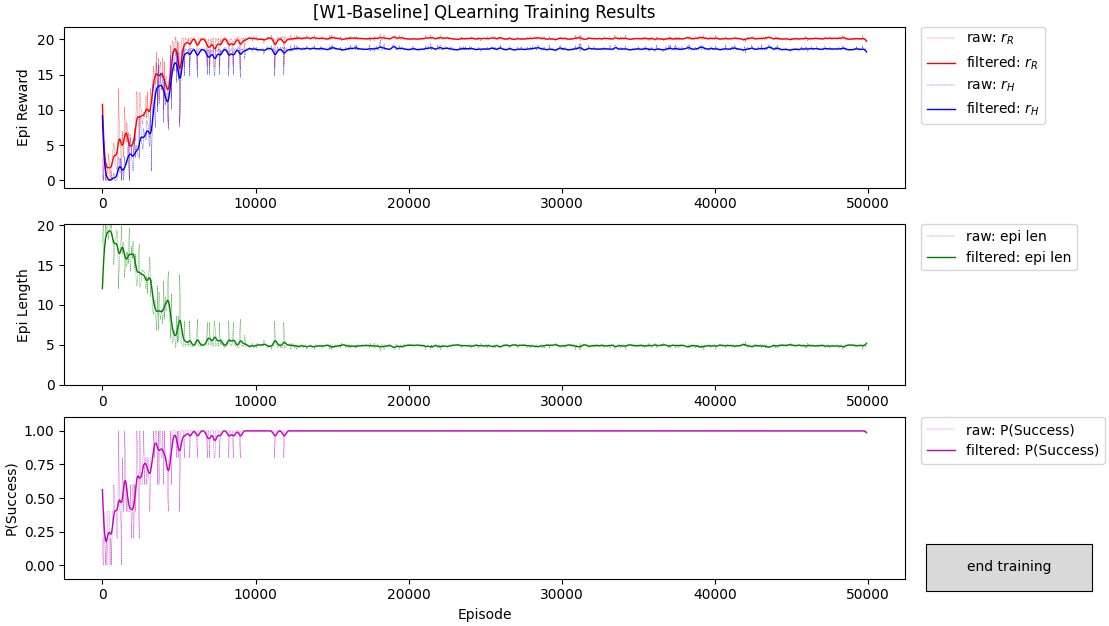
\includegraphics[width=\textwidth]{Prog4_Jan7/materials/Fig_W1_JointQ_Baseline.png}
        %      \caption{Optimal} \label{fig:W1baseline}
        %  \end{subfigure}
        %  \hfill
         \begin{subfigure}[b]{\Wfig\textwidth} \centering
             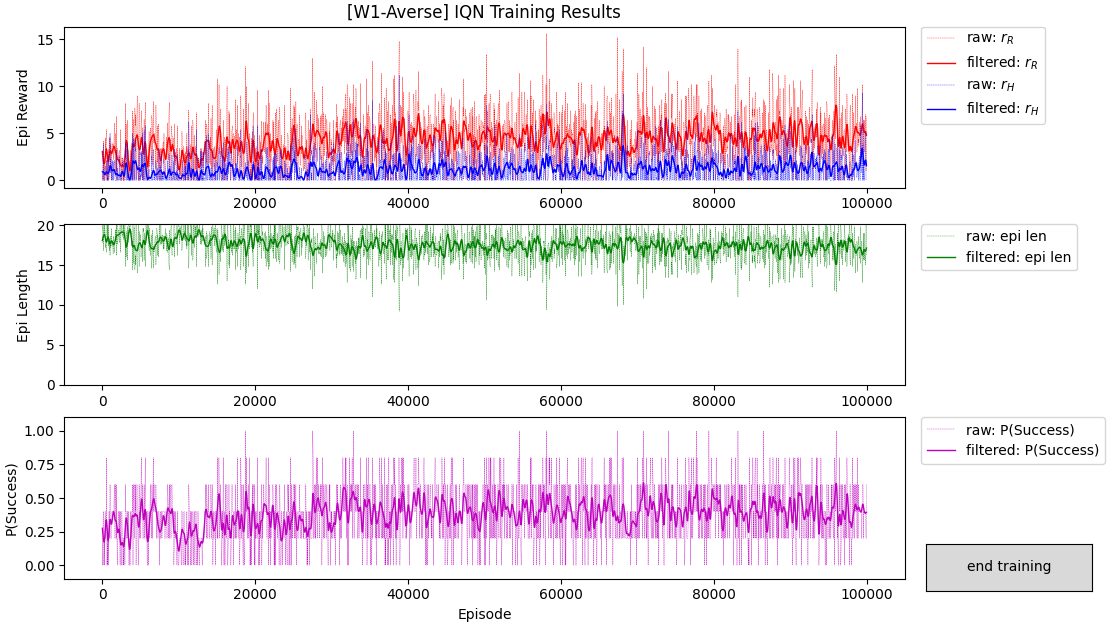
\includegraphics[width=\textwidth]{../results/IDQN_W1/Fig_W1_JointQ_Averse}
             \caption{Risk-Averse} \label{fig:W1averse}
         \end{subfigure}
         \hfill
         \begin{subfigure}[b]{\Wfig\textwidth} \centering
             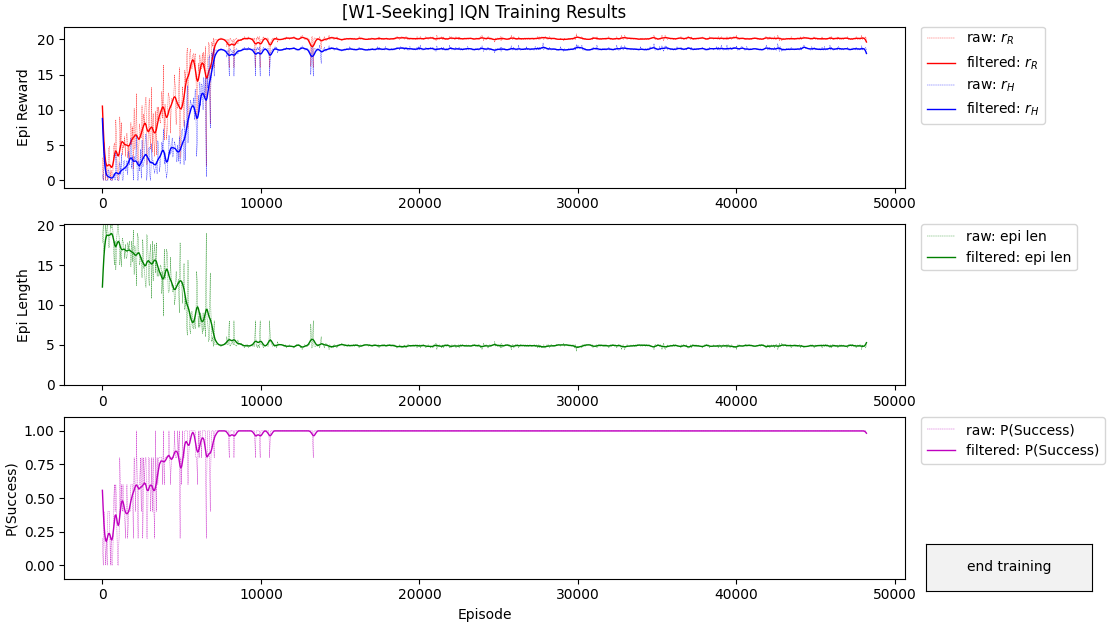
\includegraphics[width=\textwidth]{../results/IDQN_W1/Fig_W1_JointQ_Seeking}
             \caption{Risk-Seeking} \label{fig:W1seeking}
         \end{subfigure}
    \caption{World 1 Training Results}
    \label{fig:W1}
    \end{figure}
\end{frame}

\begin{frame}{Training Results (World 2)}
     \begin{figure}
     \centering
        %  \begin{subfigure}[b]{\Wfig\textwidth}  \centering
        %      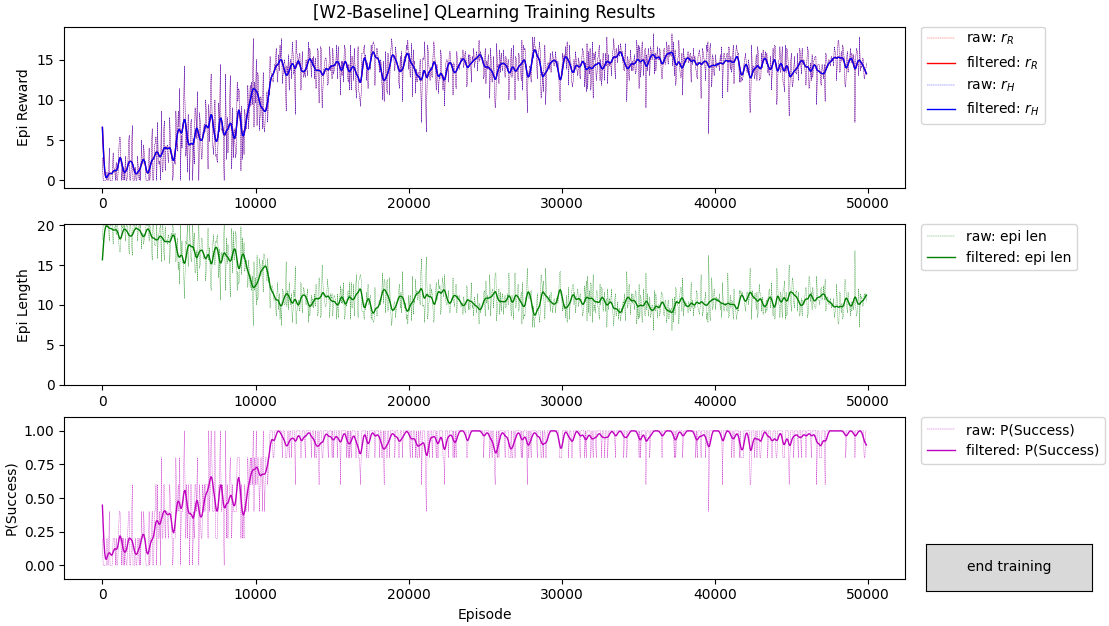
\includegraphics[width=\textwidth]{Prog4_Jan7/materials/Fig_W2_JointQ_Baseline.png}
        %      \caption{Optimal} \label{fig:W2baseline}
        %  \end{subfigure}
        %  \hfill
         \begin{subfigure}[b]{\Wfig\textwidth} \centering
             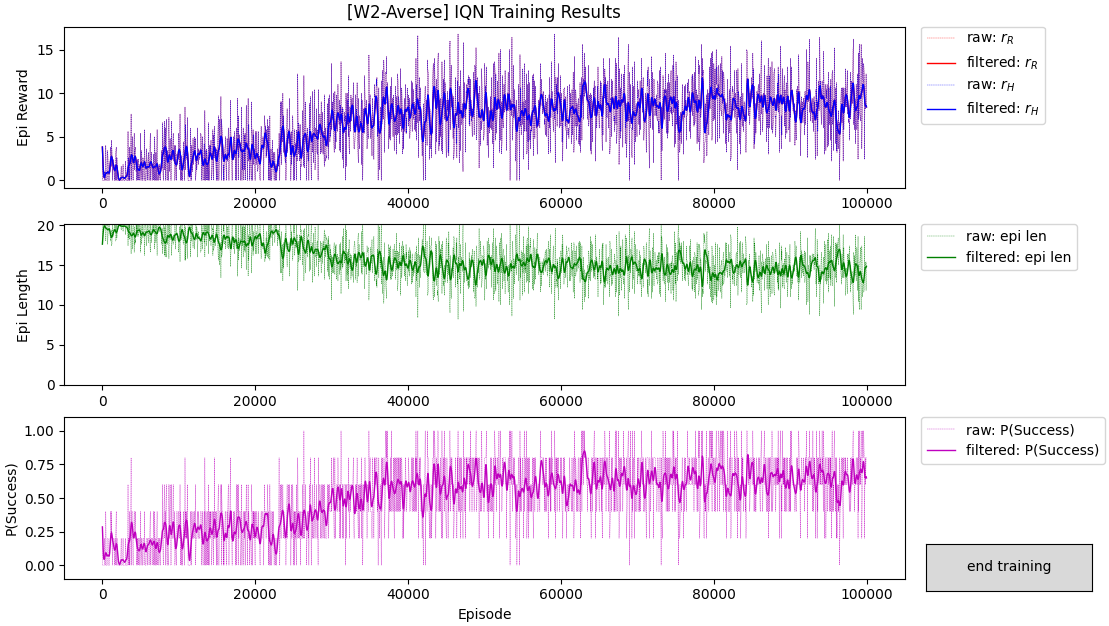
\includegraphics[width=\textwidth]{../results/IDQN_W2/Fig_W2_JointQ_Averse}
             \caption{Risk-Averse} \label{fig:W2averse}
         \end{subfigure}
         \hfill
         \begin{subfigure}[b]{\Wfig\textwidth} \centering
             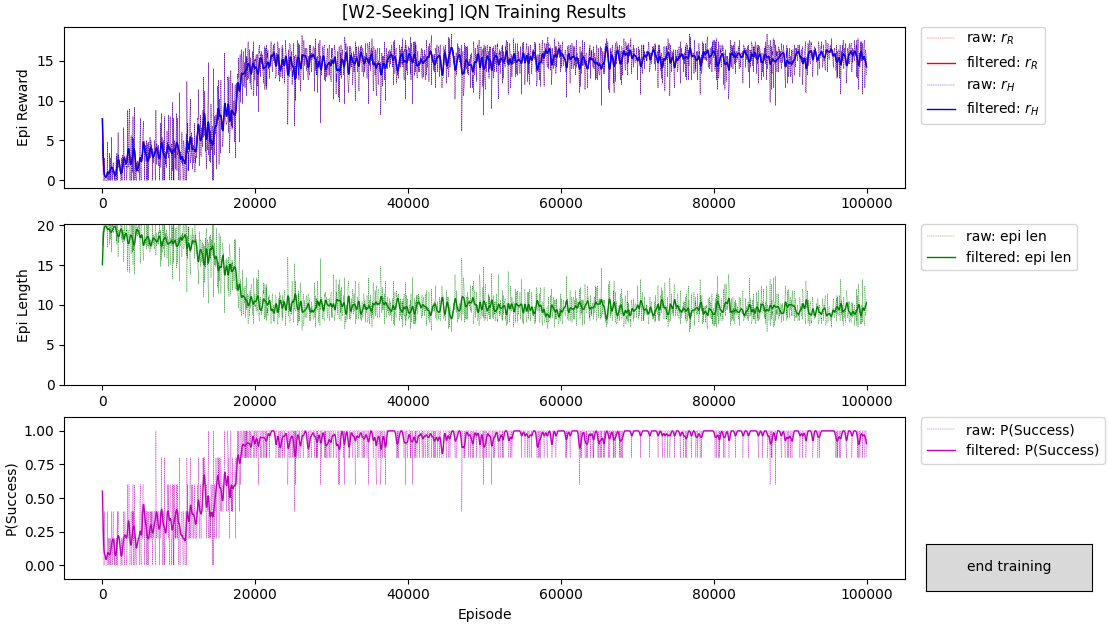
\includegraphics[width=\textwidth]{../results/IDQN_W2/Fig_W2_JointQ_Seeking}
             \caption{Risk-Seeking} \label{fig:W2seeking}
         \end{subfigure}
    \caption{World 2 Training Results}
    \label{fig:W2}
    \end{figure}
\end{frame}


\begin{frame}{Training Results (World 3)}
     \begin{figure}
     \centering
        %  \begin{subfigure}[b]{\Wfig\textwidth}  \centering
        %      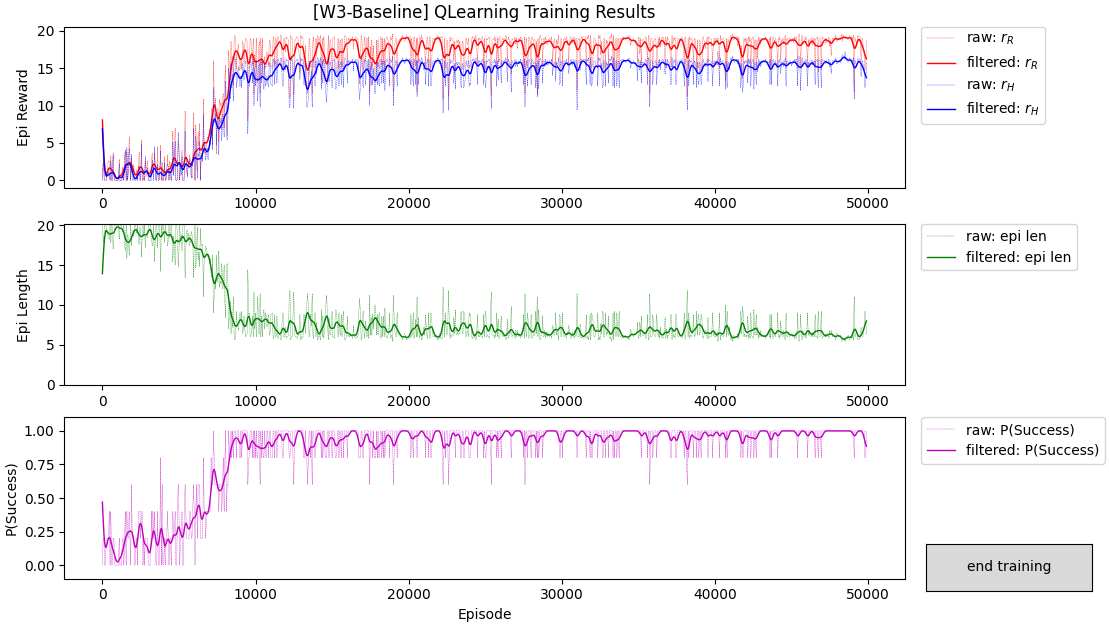
\includegraphics[width=\textwidth]{Prog4_Jan7/materials/Fig_W3_JointQ_Baseline.png}
        %      \caption{Optimal} \label{fig:W3baseline}
        %  \end{subfigure}
        %  \hfill
         \begin{subfigure}[b]{\Wfig\textwidth} \centering
             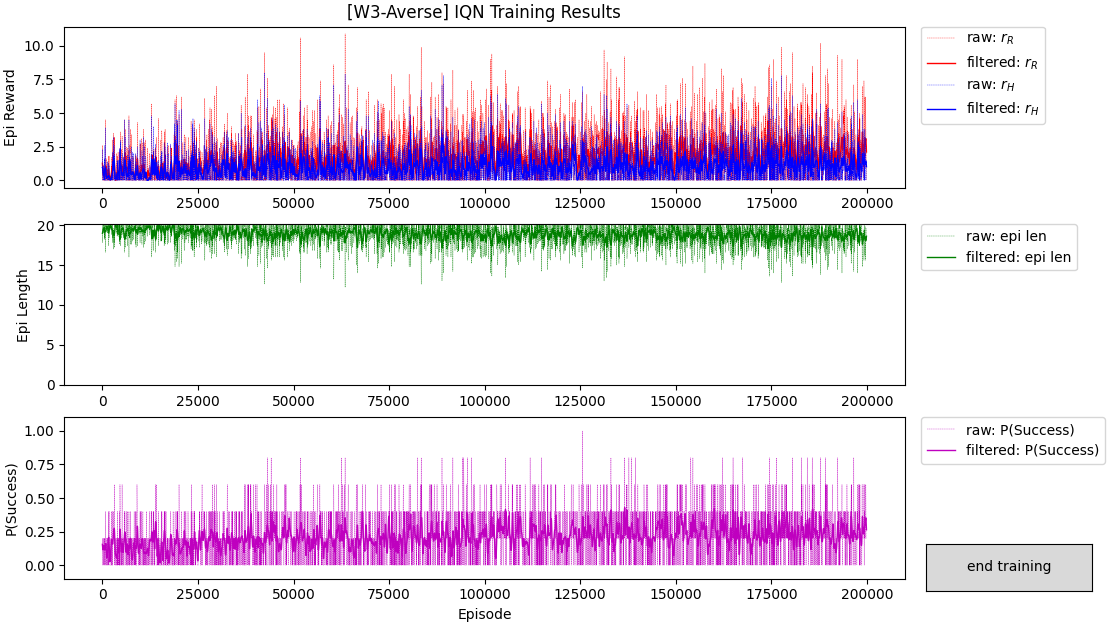
\includegraphics[width=\textwidth]{../results/IDQN_W3/Fig_W3_JointQ_Averse}
             \caption{Risk-Averse} \label{fig:W3averse}
         \end{subfigure}
         \hfill
         \begin{subfigure}[b]{\Wfig\textwidth} \centering
             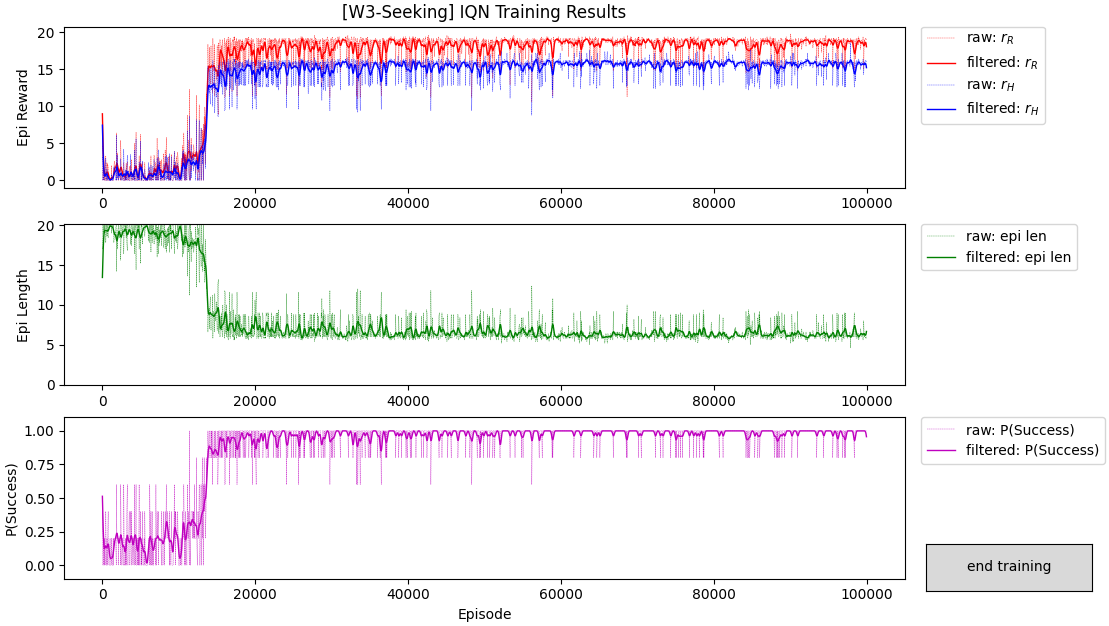
\includegraphics[width=\textwidth]{../results/IDQN_W3/Fig_W3_JointQ_Seeking}
             \caption{Risk-Seeking} \label{fig:W3seeking}
         \end{subfigure}
    \caption{World 3 Training Results}
    \label{fig:W3}
    \end{figure}
\end{frame}


\begin{frame}{Training Results (World 4)}
     \begin{figure}
     \centering
        %  \begin{subfigure}[b]{\Wfig\textwidth}  \centering
        %      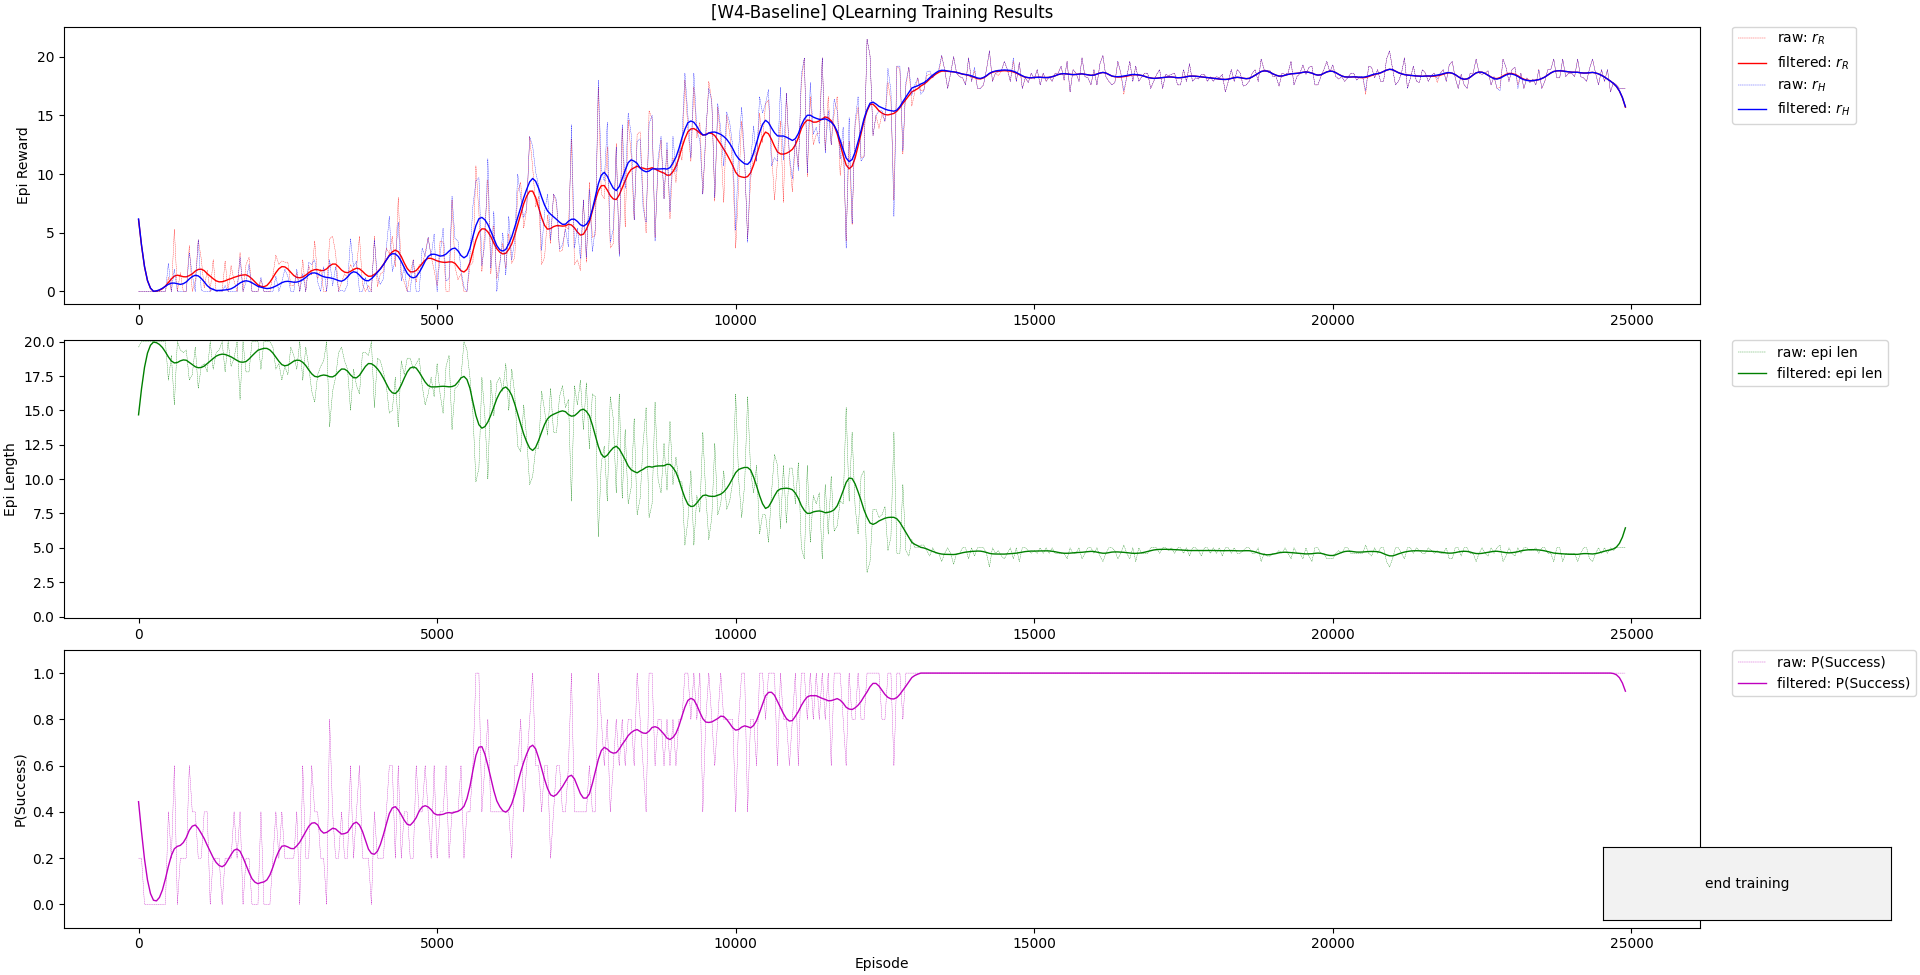
\includegraphics[width=\textwidth]{Prog4_Jan7/materials/Fig_W4_JointQ_Baseline.png}
        %      \caption{Optimal} \label{fig:W4baseline}
        %  \end{subfigure}
        %  \hfill
         \begin{subfigure}[b]{\Wfig\textwidth} \centering
             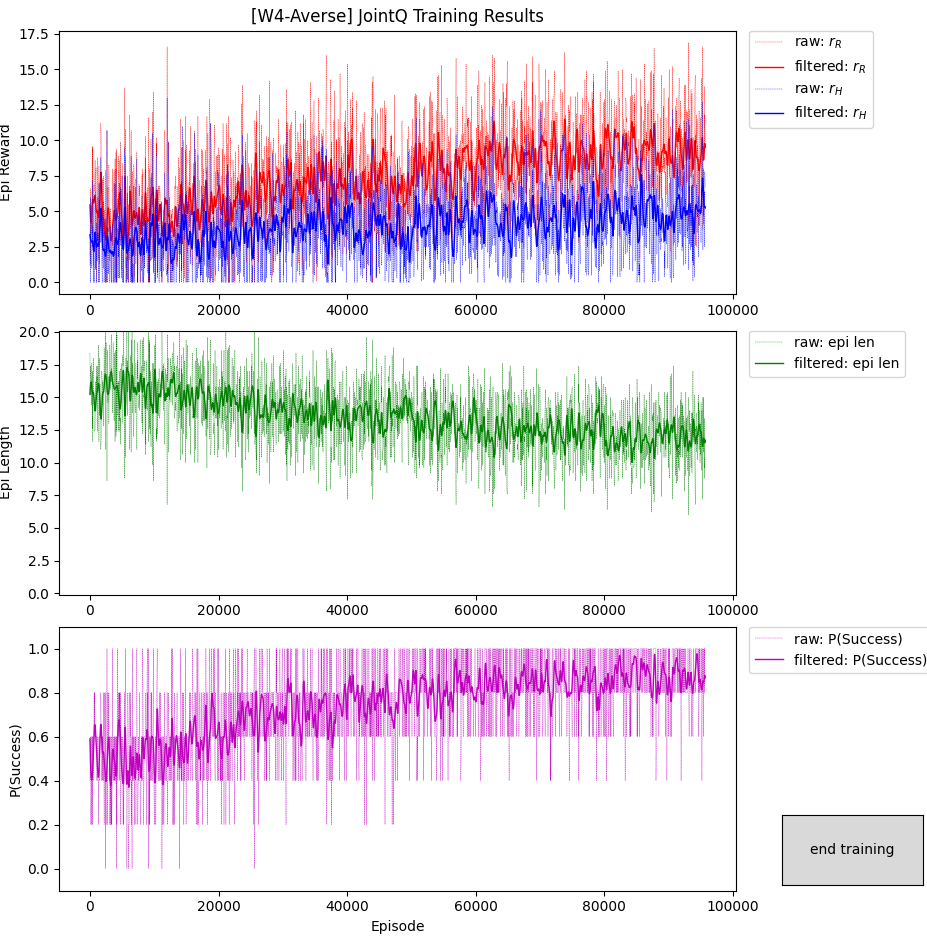
\includegraphics[width=\textwidth]{../results/IDQN_W4/Fig_W4_JointQ_Averse}
             \caption{Risk-Averse} \label{fig:W4averse}
         \end{subfigure}
         \hfill
         \begin{subfigure}[b]{\Wfig\textwidth} \centering
             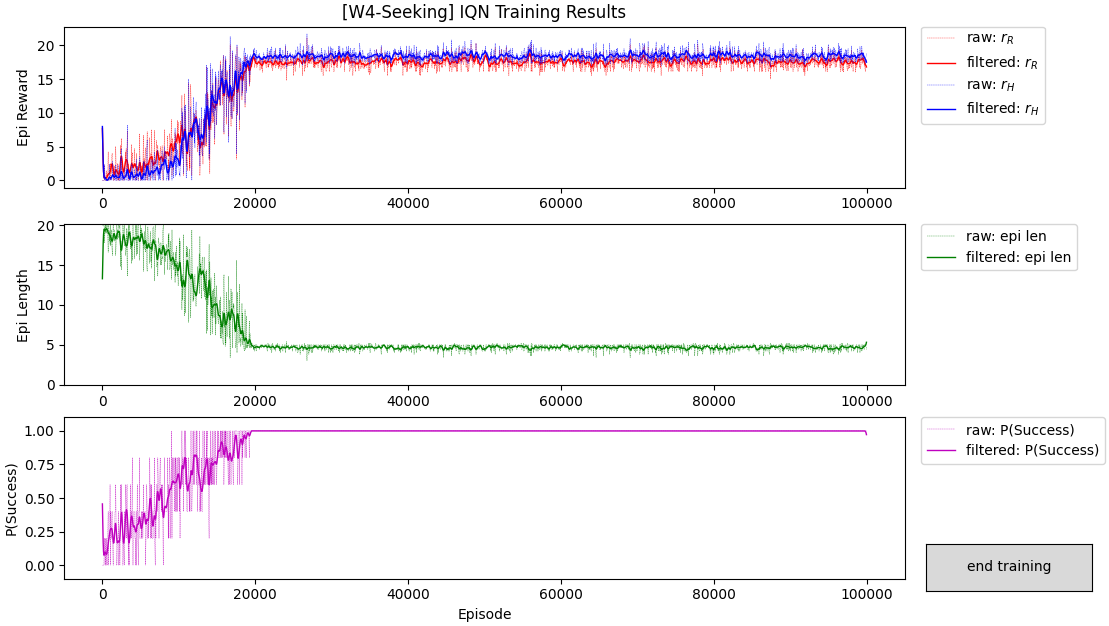
\includegraphics[width=\textwidth]{../results/IDQN_W4/Fig_W4_JointQ_Seeking}
             \caption{Risk-Seeking} \label{fig:W4seeking}
         \end{subfigure}
    \caption{World 4 Training Results}
    \label{fig:W4}
    \end{figure}
\end{frame}


\begin{frame}{Training Results (World 5)}
     \begin{figure}
     \centering
        %  \begin{subfigure}[b]{\Wfig\textwidth}  \centering
        %      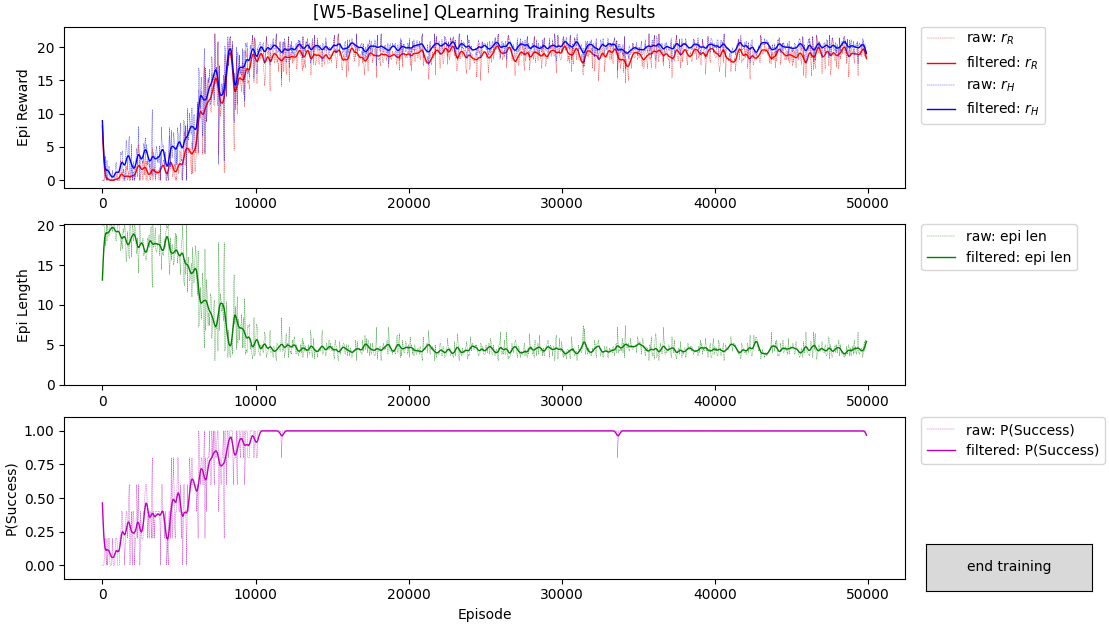
\includegraphics[width=\textwidth]{Prog4_Jan7/materials/Fig_W5_JointQ_Baseline.png}
        %      \caption{Optimal} \label{fig:W5baseline}
        %  \end{subfigure}
        %  \hfill
         \begin{subfigure}[b]{\Wfig\textwidth} \centering
             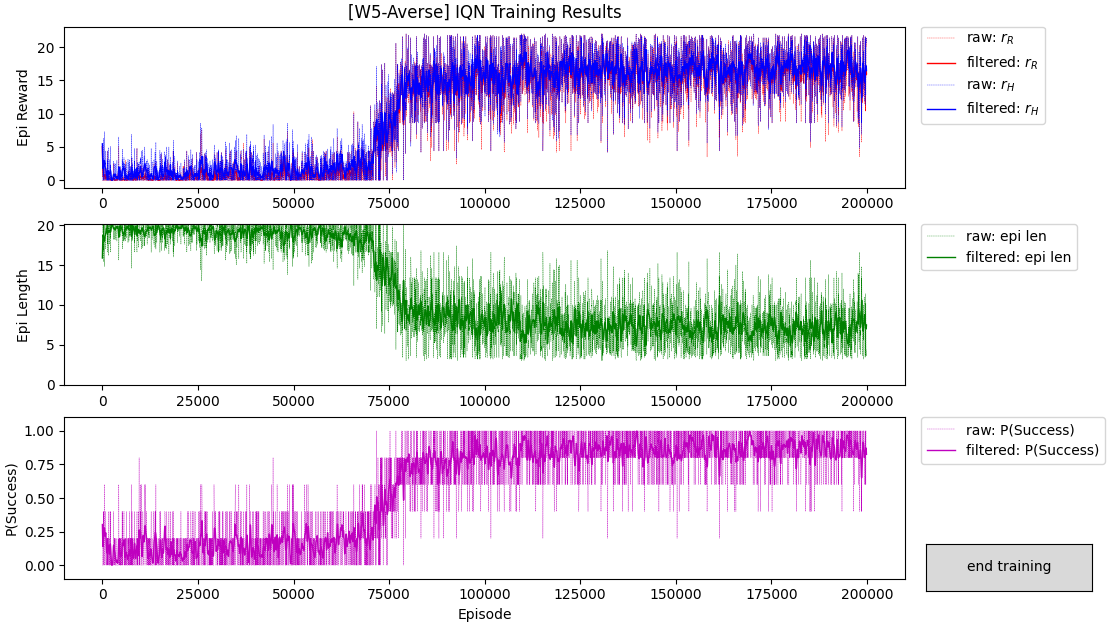
\includegraphics[width=\textwidth]{../results/IDQN_W5/Fig_W5_JointQ_Averse}
             \caption{Risk-Averse} \label{fig:W5averse}
         \end{subfigure}
         \hfill
         \begin{subfigure}[b]{\Wfig\textwidth} \centering
             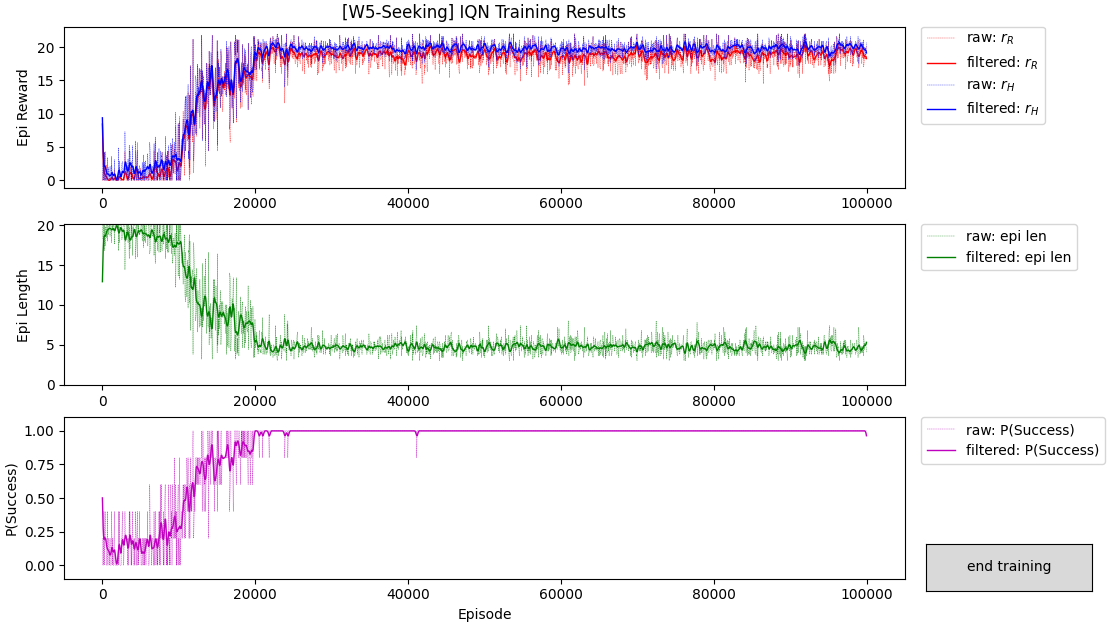
\includegraphics[width=\textwidth]{../results/IDQN_W5/Fig_W5_JointQ_Seeking}
             \caption{Risk-Seeking} \label{fig:W5seeking}
         \end{subfigure}
    \caption{World 5 Training Results}
    \label{fig:W5}
    \end{figure}
\end{frame}

\begin{frame}{Training Results (World 6)}
     \begin{figure}
     \centering
        %  \begin{subfigure}[b]{\Wfig\textwidth}  \centering
        %      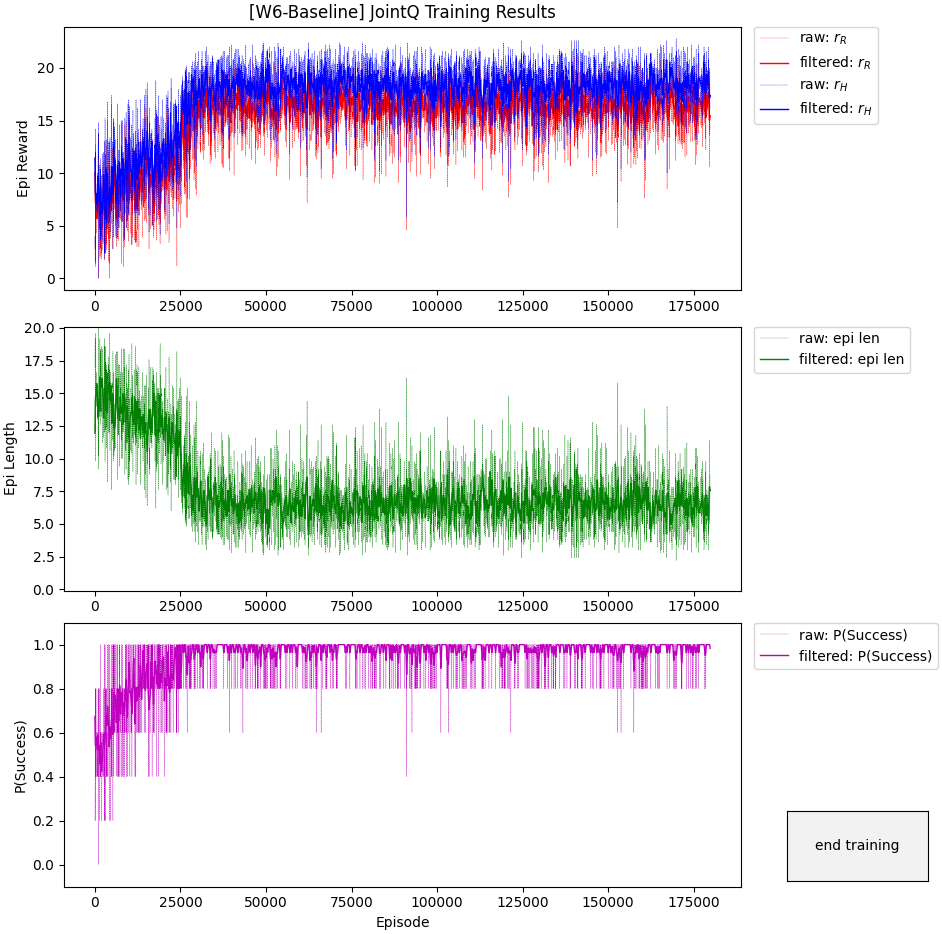
\includegraphics[width=\textwidth]{Prog4_Jan7/materials/Fig_W6_JointQ_Baseline.png}
        %      \caption{Optimal} \label{fig:W6baseline}
        %  \end{subfigure}
        %  \hfill
         \begin{subfigure}[b]{\Wfig\textwidth} \centering
             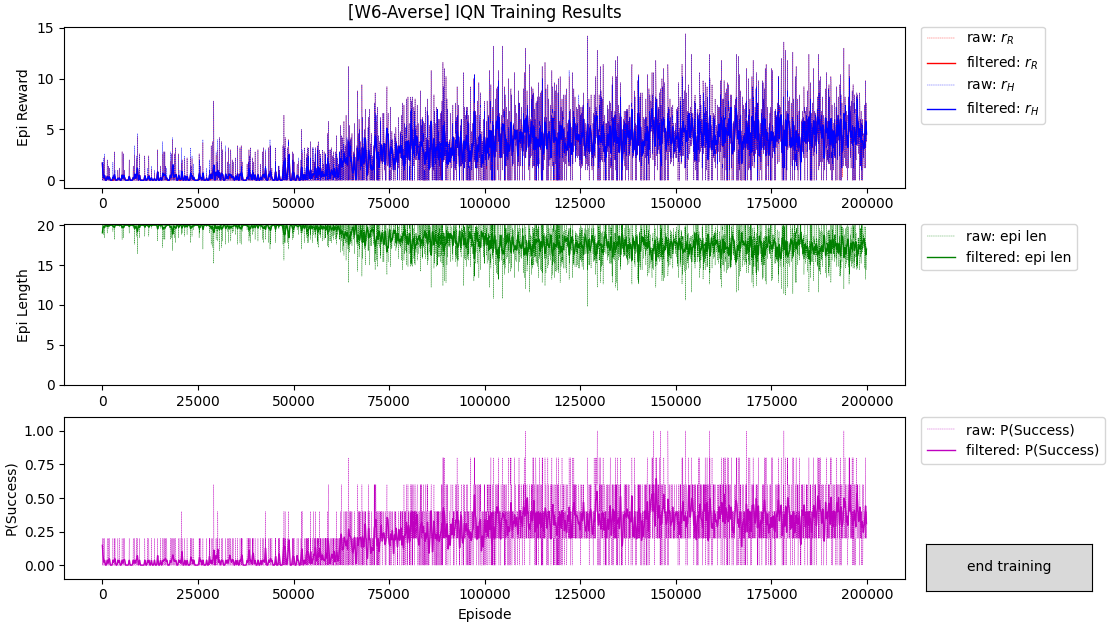
\includegraphics[width=\textwidth]{../results/IDQN_W6/Fig_W6_JointQ_Averse}
             \caption{Risk-Averse} \label{fig:W6averse}
         \end{subfigure}
         \hfill
         \begin{subfigure}[b]{\Wfig\textwidth} \centering
             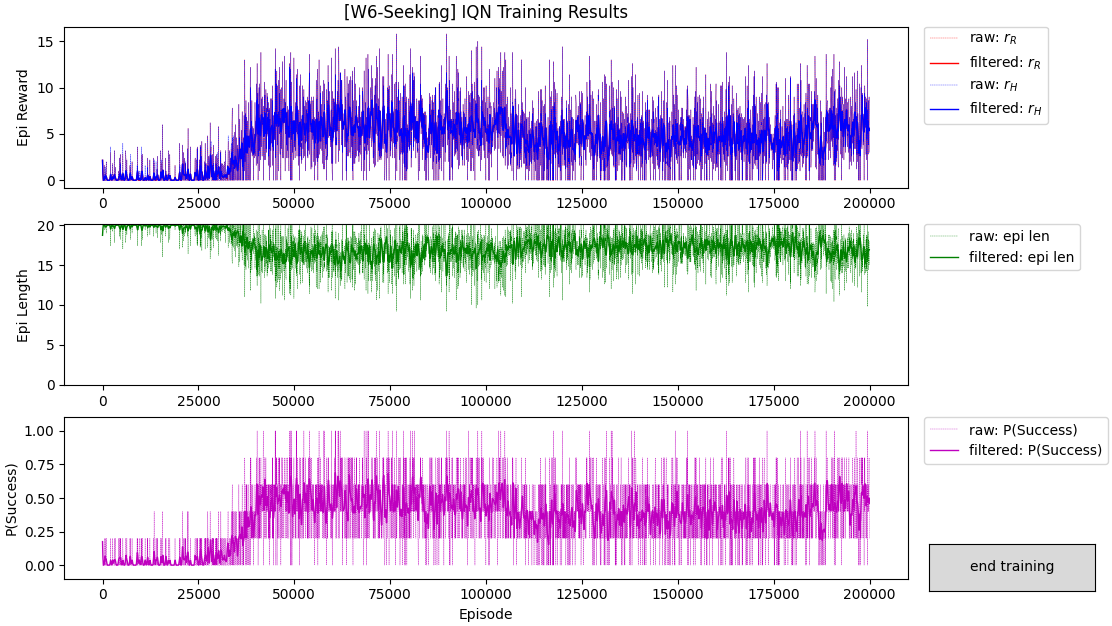
\includegraphics[width=\textwidth]{../results/IDQN_W6//Fig_W6_JointQ_Seeking}
             \caption{Risk-Seeking} \label{fig:W6seeking}
         \end{subfigure}
    \caption{World 6 Training Results}
    \label{fig:W6}
    \end{figure}
\end{frame}


 \begin{frame}{Training Results (World 7)}
      \begin{figure}
      \centering
%          \begin{subfigure}[b]{\Wfig\textwidth}  \centering
%              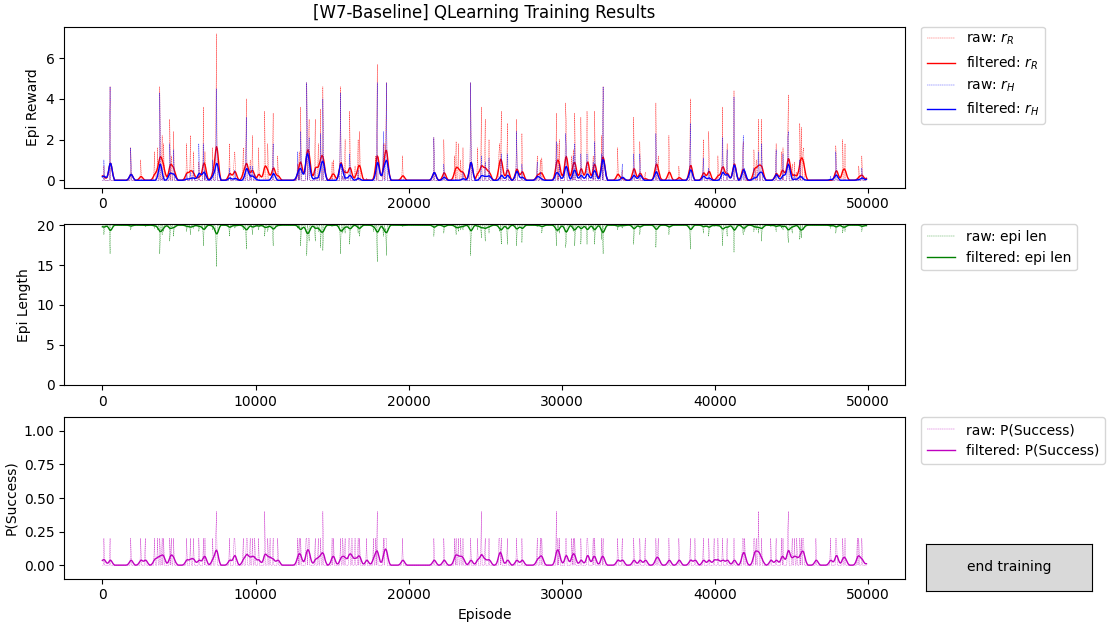
\includegraphics[width=\textwidth]{Prog4_Jan7/materials/Fig_W7_JointQ_Baseline.png}
%              \caption{Optimal} \label{fig:W7baseline}
%          \end{subfigure}
%          \hfill
          \begin{subfigure}[b]{\Wfig\textwidth} \centering
              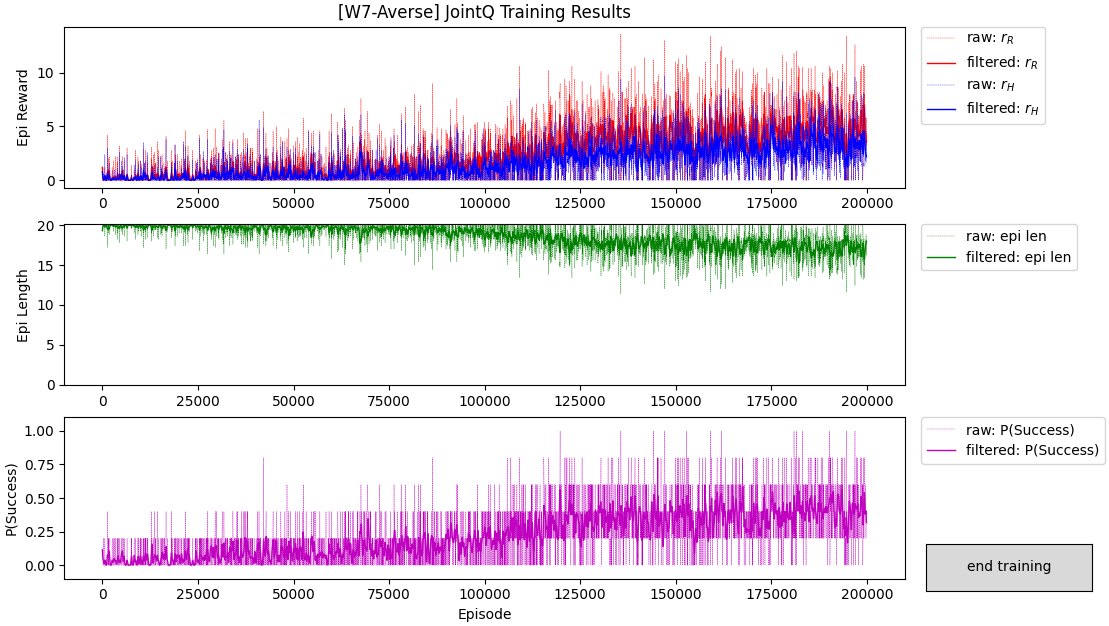
\includegraphics[width=\textwidth]{../results/IDQN_W7//Fig_W7_JointQ_Averse}
              \caption{Risk-Averse} \label{fig:W7averse}
          \end{subfigure}
          \hfill
          \begin{subfigure}[b]{\Wfig\textwidth} \centering
              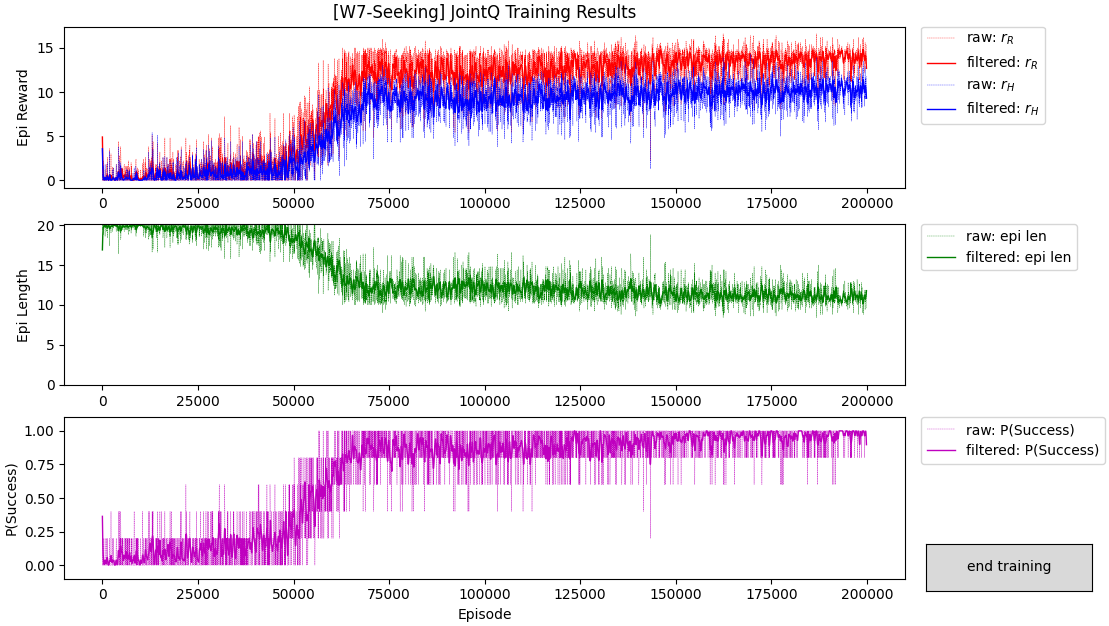
\includegraphics[width=\textwidth]{../results/IDQN_W7/Fig_W7_JointQ_Seeking}
              \caption{Risk-Seeking} \label{fig:W7seeking}
          \end{subfigure}
     \caption{World 7 Training Results}
     \label{fig:W7}
     \end{figure}
 \end{frame}


\subsection{Discussion}\label{subsec:discussion}\begin{frame}{Discussion}
\begin{itemize}
    \item Policies are generally noisy due to
    \begin{itemize}
        \item non-stationarity
        \item rationality constant = 1
    \end{itemize}
    \item Equilibrium would be less stochastic with higher rationalities
    \item Noise in final result pseudo-required to avoid the previously mentioned all or nothing problem
        \footnonte{e.i. there exists dis-coordination and vulnerability to partner uncertainty}
    \item Baseline (optimal) $\pi_0$ policies are often similar to Risk-Seeking $\pi_S$ policies since the game is designed for the agents to succeed
    \begin{itemize}
        \item Rushing through penalties is often a good strategy
        \item $\pi_S$ still more susceptible to partner and target stochasticity
    \end{itemize}
    \item \textit{*may make minor attempts to improve policies in future but this is good for now}
\end{itemize}
\end{frame}
%#########################################################
%#########################################################
%#########################################################
\section{Simulation}\label{sec:simulation} \displayTOC
\subsection{Formulation}
\begin{frame}{Simulation Setup}
    Goal: \begin{itemize}
        \item Evaluate how assumptions of H's risk-sensitivity effect team performance
        \item Provide validation that there are differing or conflicting optimal policies based on risk-sensitivity
    \end{itemize}
    Experimental Conditions: \begin{itemize}
        \item We manipulate
        \begin{itemize}
            \item what R assumes H's policy to be ($\hat{\pi}_{H}$)
            \item what H's policy actually is ($\pi_{H}$)
        \end{itemize}
        \item The experimental condition is then written as $\cond[H][H]$
        \begin{itemize}
             \item superscript is R's assumption of H policy
             \item subscript is H's actual policy
            \item no script denotes all possible combinations of the missing index
            \begin{itemize}
                \item e.i. $\cond[][A] =\cond[A][A] \cup \cond[S][A]$
            \end{itemize}
        \end{itemize}

    \end{itemize}
\end{frame}
\begin{frame}{Simulation Setup}
    Experimental Conditions: \begin{itemize}
        \item Therefore, we get four experimental conditions $\cond$:
        \begin{itemize} \vspace{10}
            \item $\cond[A][A]$: Assume-Averse + Is-Averse   (Correct Assumption) \vspace{10}
            \item $\cond[S][A]$: Assume-Seeking + Is-Averse  (Incorrect Assumption) \\
            \item[]
            \item $\cond[A][S]$: Assume-Averse + Is-Seeking  (Incorrect Assumption) \\
            \item[]
            \item $\cond[S][S]$: Assume-Seeking + Is-Seeking (Correct Assumption) \\
            \item[]
            \item \textit{two baseline policies are also used $\cond[0][0]$ for reference}
        \end{itemize}
    \end{itemize}
\end{frame}

\begin{frame}{Simulation Analysis}
    Approach: \begin{itemize}
        \item We \textbf{only compare between R's assumption} and within H's actually policy
        \item H's actually policy directly effects game performance and invalidates some evaluation metrics
        \item R's policy will be $\pi_R=\pi_0$ conditioned on $\hat{\pi}_{H}$ using \ac{QRE}
        \item H will assume R uses H's true policy $\hat{\pi}_{R}=\pi_{H}$
        \item Run simulated game 1000x for each of the 4 conditions
    \end{itemize}
\end{frame}

\begin{frame}{Simulation Analysis}
    Performance Metrics: \begin{itemize}
        \item Agent's Mean Cumulative Reward $\sum_{t}^{T} R_{(k,t)} \forall k \in K $
        \item Team's Mean Cumulative Reward $\sum_{t}^{T} \bar{R}_{t}  $
        \item Mean Episode Length $|T|$ \footnote{Moves until catching the target or game duratio expiring}
        \item Number of penalty states $S_{\rho}$ entered $\sum_{t\in T} \Ind\{s_{(k,t)} \in S_{\rho} \} \forall k \in K$
        \item Probability of catching target $p(catch)$
        \item Accuracy in $k$'s MM of partner $-k$ $\hat{p}(a_{(-k,t)}|\hat{\pi}_{-k}(s_t))$ \footnote{Also the mean probability of observing $-k$'s action}
    \end{itemize}
    Insight:
    \begin{itemize}
        \item How well are agents and team performing
        \item What are agent's prefernce for entering penalty states
        \item How well do agents understand each other
    \end{itemize}
\end{frame}


\subsection{Simulation Hypothesis}\label{subsec:simulation-hypothesis}
\begin{frame}{Simulation Hypothesis}
    When R assumes wrong ($\cond ^{\hat{\pi}_H \neq \pi_H}_{\pi_H}$) for all $\pi_H \in (\pi_A,\pi_S)$: % due to discoordination
    \begin{itemize}
        \item[]
        \begin{itemize}
            \item[\textbf{H1.1}:] Each agent's and team reward will decrease
            \item[\textbf{H1.2}:] Episode length will increase
            \item[\textbf{H1.3}:] Probability of catching target will decrease
            \item[\textbf{H1.3}:] Number of penalty states entered will increase
            \item[\textbf{H1.4}:] Both agents will not be able to predict each other's actions well (small  $p(a_{-k} | \hat{\pi}_{-k})$)
        \end{itemize}
    \end{itemize}
    When H is averse ($\pi_H = \pi_A$) instead of seeking: % due to discoordination
    \begin{itemize}
        \begin{itemize}
            \item[\textbf{H2.1}:] Magnitude of performance losses will be less significant
            \item[\textbf{H2.2}:] Performance will be worse than if $\cond[][S]$%$\pi_H = \pi_S$
            % \item[\textbf{H2.3}:]
            % \item[\textbf{H2.3}:]
        \end{itemize}
    \end{itemize}
    Misc. Hypothesises
    \begin{itemize}
        \begin{itemize}
            \item[\textbf{H3}:] Only minor changes in terminal state location will occur when agents succeed (e.i. objective remains the same but joint-trajectory changes).
        \end{itemize}
    \end{itemize}
\end{frame}








\subsection{Results}

%\newcommand{\cond}[2]{\mathcal{C}^{\hat{\pi}_{#1}}_{\pi_{#2}}} %_{(\hat{#1},#2)}

%\newcommand{\cond}[2][][]{
%    \ifthenelse { \equal{#1}{} }  %if short caption not specified, use long caption (no slant)
%        {\mathcal{C}_{\pi_{#2}}}   % if #1 == blank
%        {\mathcal{C}^{\hat{\pi}_#1}_{\pi_{#2}} }   % else (not blank)
%}



\begin{frame}{Simulation Results}
    Reading Plots:
    \begin{itemize}
        \item * on top of bars and in key indicate correct assumption made
        \item optimal policy $\cond[0][0]$ given for reference %$(\hat{pi}_{0} \times \pi_{0})$
        \item comparison between correct and incorrect R assumptions grouped between fixed $\pi_H$
    \end{itemize}
\end{frame}


\begin{frame}{Simulation Results (World 1)}
     \begin{figure} \centering
        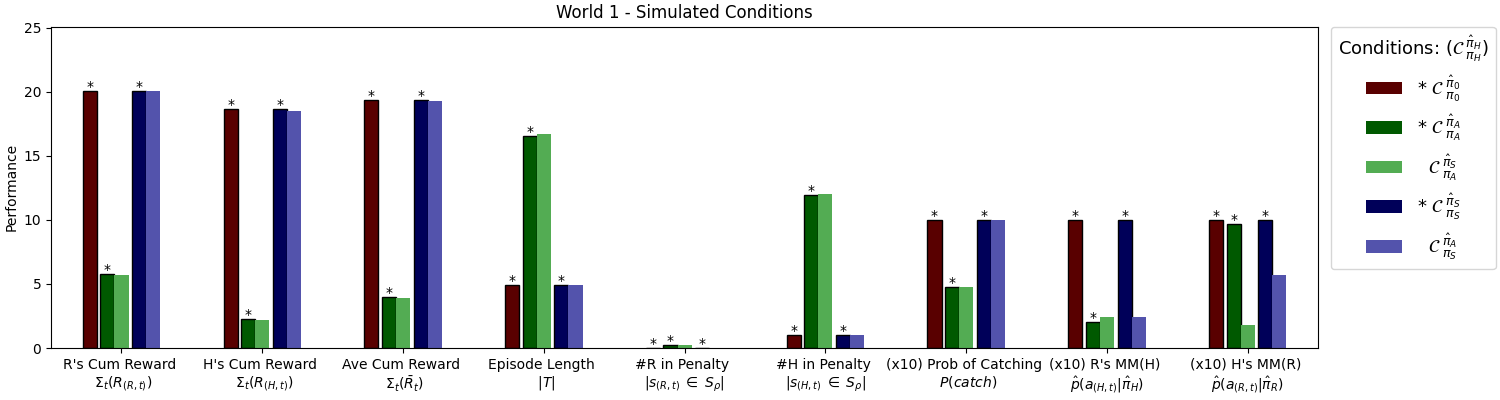
\includegraphics[width=0.99\textwidth]{../results/policy_comparisons/Fig_AssumptionComparison_W1}
        \caption{Evaluation of simulated conditions for World 1}
        \label{fig:PolicyCompW1}
    \end{figure}
\end{frame}

\begin{frame}{Simulation Results (World 2)}
     \begin{figure} \centering
        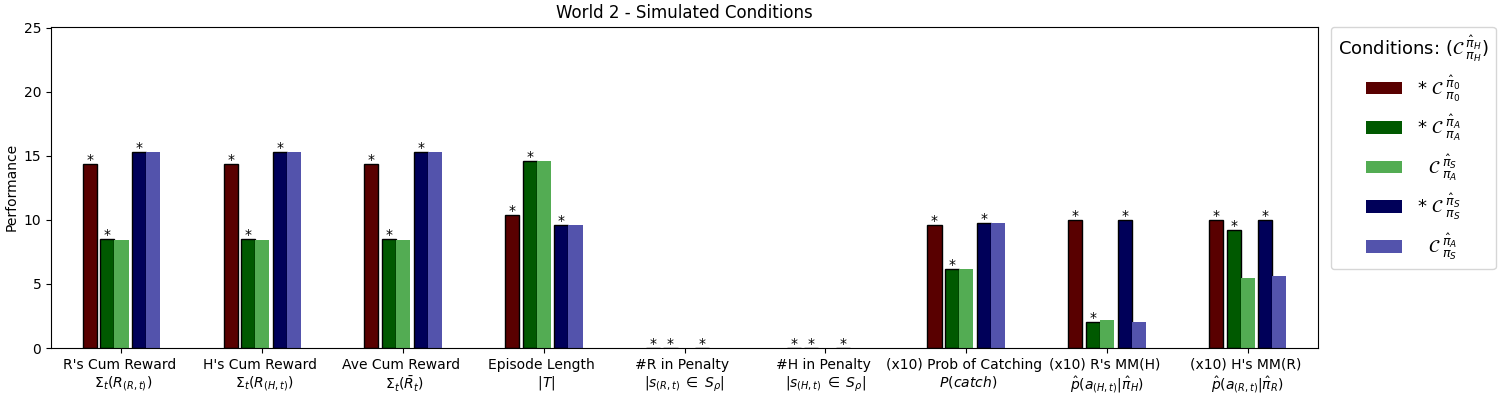
\includegraphics[width=0.99\textwidth]{../results/policy_comparisons/Fig_AssumptionComparison_W2}
        \caption{Evaluation of simulated conditions for World 2}
        \label{fig:PolicyCompW2}
    \end{figure}
\end{frame}

\begin{frame}{Simulation Results (World 3)}
     \begin{figure} \centering
        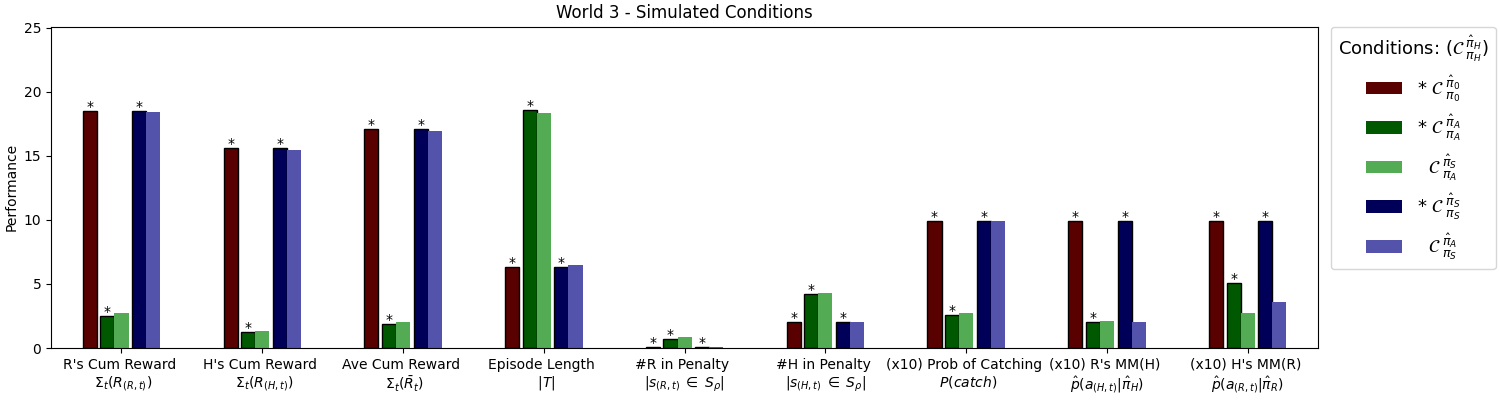
\includegraphics[width=0.99\textwidth]{../results/policy_comparisons/Fig_AssumptionComparison_W3}
        \caption{Evaluation of simulated conditions for World 3}
        \label{fig:PolicyCompW3}
    \end{figure}
\end{frame}

\begin{frame}{Simulation Results (World 4)}
     \begin{figure} \centering
        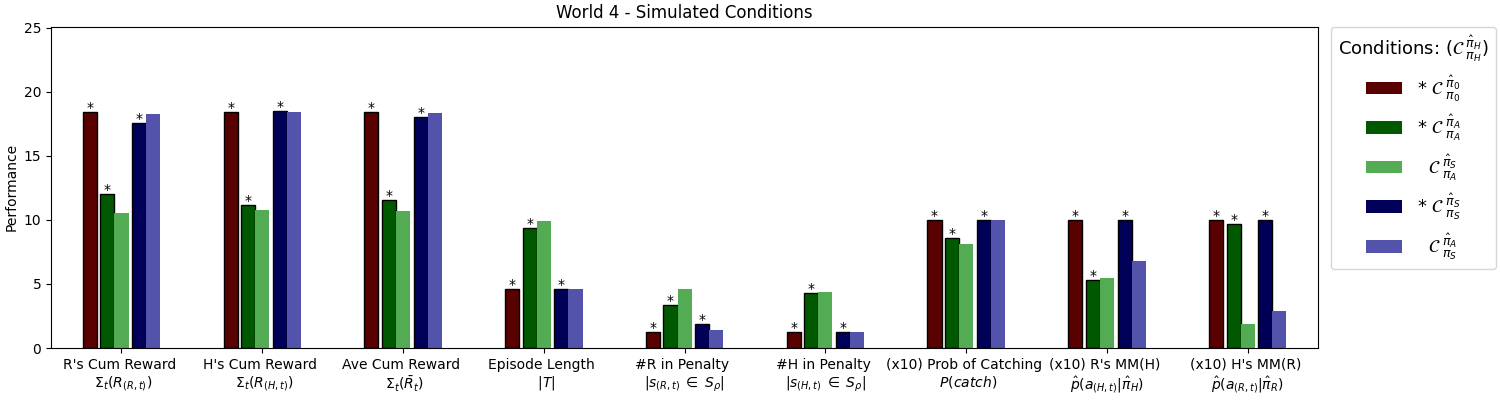
\includegraphics[width=0.99\textwidth]{../results/policy_comparisons/Fig_AssumptionComparison_W4}
        \caption{Evaluation of simulated conditions for World 4}
        \label{fig:PolicyCompW4}
    \end{figure}
\end{frame}

\begin{frame}{Simulation Results (World 5)}
     \begin{figure} \centering
        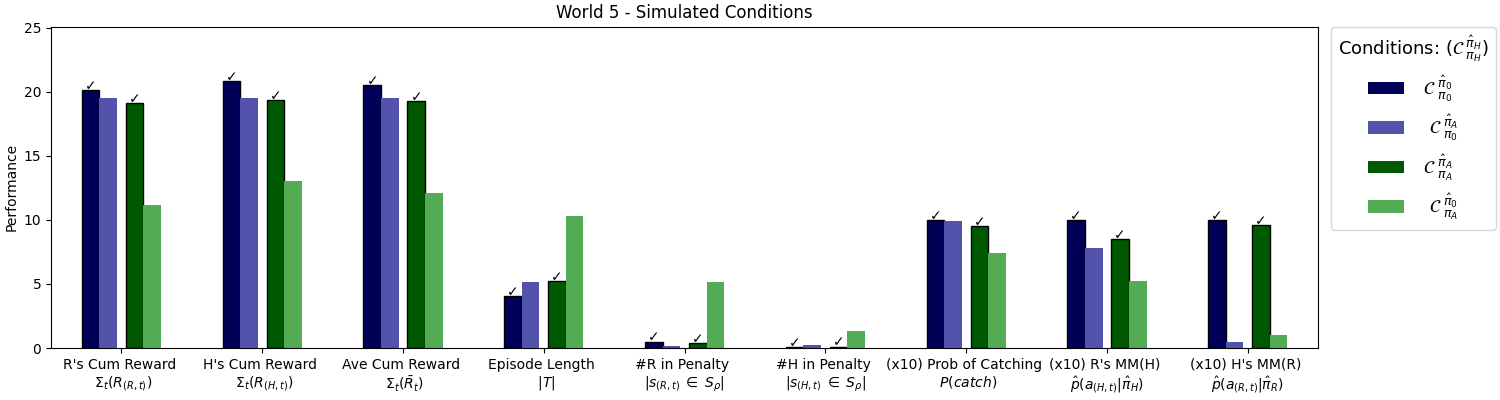
\includegraphics[width=0.99\textwidth]{../results/policy_comparisons/Fig_AssumptionComparison_W5}
        \caption{Evaluation of simulated conditions for World 5}
        \label{fig:PolicyCompW5}
    \end{figure}
\end{frame}


\begin{frame}{Simulation Results (World 6)}
     \begin{figure} \centering
        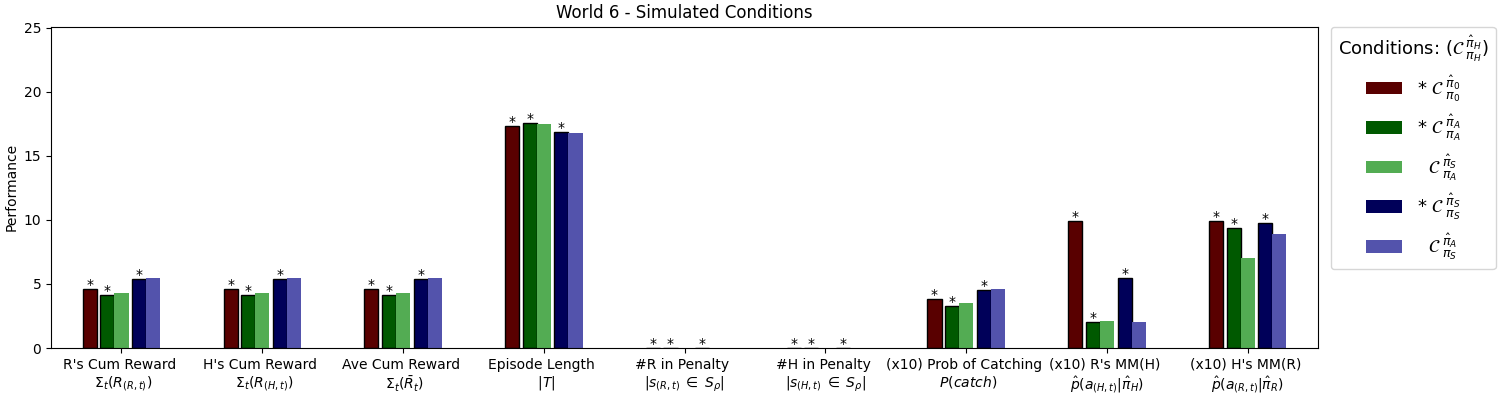
\includegraphics[width=0.99\textwidth]{../results/policy_comparisons/Fig_AssumptionComparison_W6}
        \caption{Evaluation of simulated conditions for World 6}
        \label{fig:PolicyCompW6}
    \end{figure}
\end{frame}

\begin{frame}{Results (World 7)}
     \begin{figure} \centering
        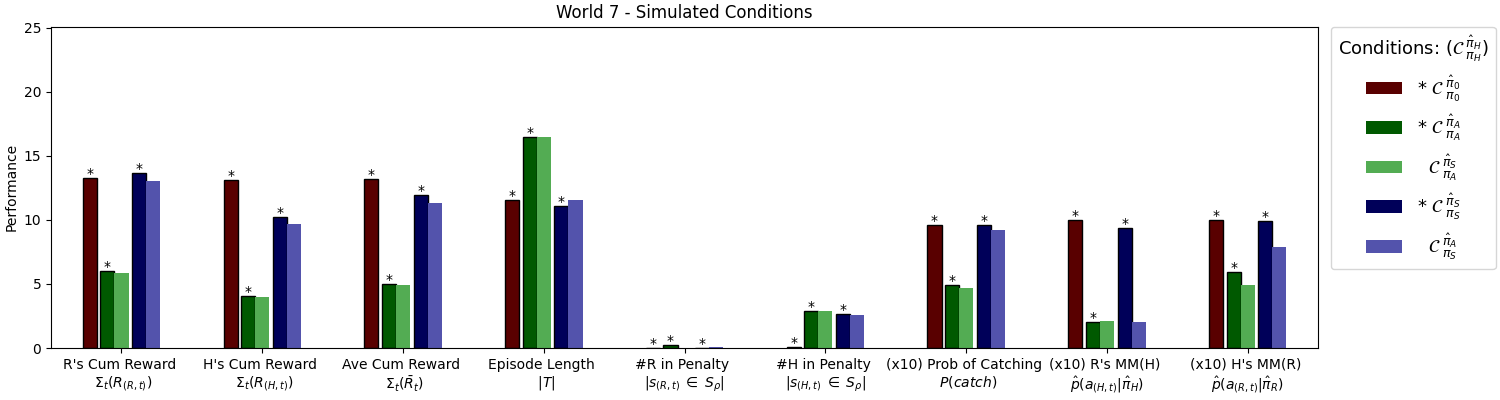
\includegraphics[width=0.99\textwidth]{../results/policy_comparisons/Fig_AssumptionComparison_W7}
        \caption{Evaluation of simulated conditions for World 7}
        \label{fig:PolicyCompW7}
    \end{figure}
\end{frame}

\begin{frame}{Simulation Results (Mean)}
     \begin{figure} \centering
        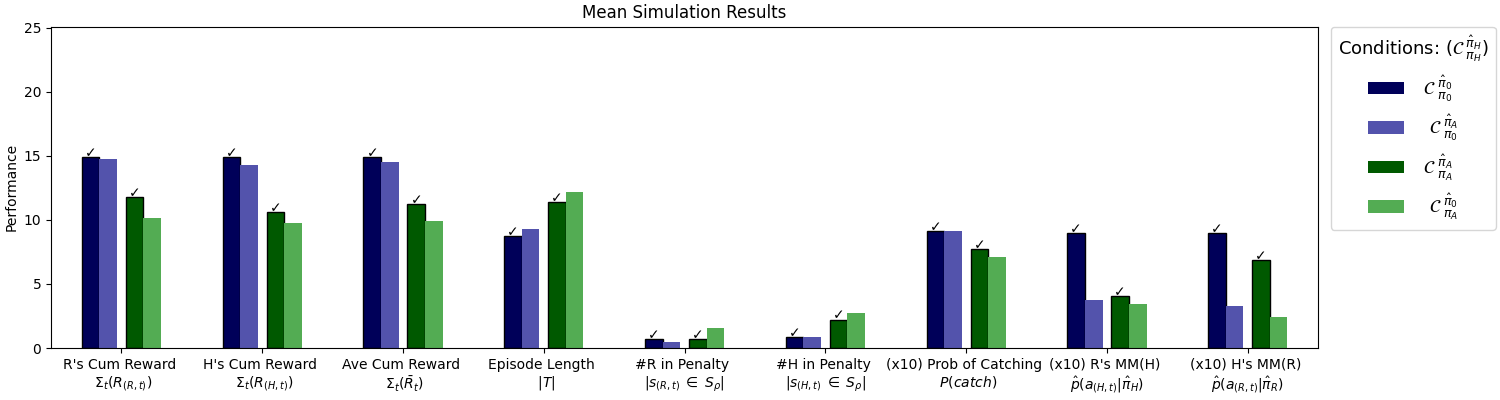
\includegraphics[width=0.99\textwidth]{../results/policy_comparisons/Fig_AssumptionComparison_Summary}
        \caption{Evaluation of simulated conditions summary}
        \label{fig:PolicyCompSummary}
    \end{figure}
\end{frame}

\subsection{Discussion}

\begin{frame}{Observations}
        \textbf{Observation 1:} Similar performances in baseline $\pi_H = \pi_0$ and risk-seeking $\pi_H = \pi_S$ human conditions:
        \begin{itemize}
            \item Minimal losses in $\sum r_t$, epi length $T$, and $p(catch)$ when H is risk-seeking $\pi_S$ relative to when H is optimal  $\pi_0$
%            \item $(\hat{\pi}_0 \times \pi_0) \approx (\hat{\pi}_S \times \pi_S ) \approx  (\hat{\pi}_A \times \pi_S)$
            \item worlds designed with simple, achievable catches in mind
            \item therefore, best strategy is often to rush straight towards target
            \item realized trajectories $\zeta_t$ are then similar $\zeta(\pi_0)_t \approx \zeta(\pi_S)_t$
            \item risk-seeking $\pi_S$'s effect on rewards
            \begin{itemize}
                \item for true cumulative rewards (seen in figures) $\sum r(\pi_0)_t \approx \sum r(\pi_S)_t $
                \item However, H's perceived reward $\sum \tilde{r}(\pi_0)_t < \sum \tilde{r}(\pi_S)_t$ due to the discounted penalties
            \end{itemize}
            \item Coordination effects diminish as we get closer to the target
            \begin{itemize}
                \item If my action is obvious (by mere virtue of being closer to the target), I do not need to model your behavior
                    \footnote{e.i. does not matter what I assume if we are 1 move away from the target}
                \item Opportunity for the incorrect assumption to affect coordination is small when $\pi_H = \pi_S$
            \end{itemize}
        \end{itemize}
\end{frame}

\begin{frame}{Observations}
    \textbf{Observation 2:} Agent Rewards, Team Rewards, and Episode Length
    \begin{itemize}
        \item Sizable performance losses when $\cond[A][A] \rightarrow \cond[S][A]$
        \item Negligible difference when $\cond[S][S] \rightarrow \cond[A][S]$  as described by discussion in Observation 1
        \item Higher cumulative rewards for R is product of game design, not policy assumption
    \end{itemize}

    \textbf{Observation 3:} \# of Penalty States Entered
    \begin{itemize}
        \item High number of penalty states entered by R when $\cond[S][A] $
        \item R assumes H will rush straight towards the target but H does not
        \item R therefore has to idle or move about in penalty states to wait for H to approach
    \end{itemize}
\end{frame}

\begin{frame}{Observations}
    \textbf{Observation 4:} Accuracy of Agent's Mental Model (MM(Partner))
    \begin{itemize}
        \item Both MM's of their partner saw significant losses in all $\cond[][]$
        \item H's MM(R) more significant losses than when $\cond[A][A] \rightarrow \cond[S][A]$
        \item R's MM(H) was more accurate in the $\cond[0][0]$ than when $\cond[S][S]$
        \item Baseline $\pi_0$ had best prediction accuracy in MM
        \item Generally, agents found partner's actions harder to predict
        \footnote{This supports Observation 1 in that effective coordination in MM's can significantly decrease
        with little loss in task performance by mere virtue of being closer to the target}
        \item Has implications for trust degradation (process information)
    \end{itemize}

\end{frame}


\newcommand{\rawcond}[2]{\mathcal{C}^{#1}_{#2}}

\begin{frame}{Discussion}
    Summary:
    \begin{itemize}
        \item Expected effects of correct vs incorrect assumption for $\cond[][A]$ in all categories
        \item Expected effects of correct vs incorrect in MM of partner actions for all $\cond[][]$
        \item Unexpected negligible losses in reward, episode length and $p(catch)$ for $\cond[][S]$
        \item Unexpected similarity between $\cond[0][0]$, $\cond[S][S]$, and $\cond[A][S]$ policies
    \end{itemize}
    Implication:
    \begin{itemize}
        \item Trust as process information likely affected in all $\cond[][]$
        \item Trust as performance information likely affected when $\cond[][A]$
            \footnote{Would like to see more coordination effect when  $\cond[][S]$ but this is exceedingly challenging with a approxitaley rational target}
        \item Sufficient effect in coordination to evaluate trajectories when $\cond[][A]$
    \end{itemize}
\end{frame}
%#########################################################
%#########################################################
%#########################################################

\section{Ongoing Work} \displayTOC
\subsection{Web-Server}
\begin{frame}{Web-Server}
    Status: \begin{itemize}
        \item Game is functioning with all policy conditions
        \item Hosting multiple concurrent users available
        \item Data collection system is validated
    \end{itemize}
    Challenges: \begin{itemize}
        \item ISP does not want me hosting website on private network
        \item ASU will not allow hosting
    \end{itemize}
    Open Items: \begin{itemize}
        \item Need a long-term web hosting solution (security and ISP compatibility)
        \item Likely need to purchase a web host service if ISP reaches out
        \item Might be a good idea anyway since I am bootlegging a non-http port for http
    \end{itemize}
\end{frame}

\subsection{Final Pretrial Validation}
\begin{frame}{Final Pretrial Validation}
    Status:
    \begin{itemize}
        \item Can test in parallel with final web-server items
        \item Intend to see if conditions are comparable compared to simulation
        \item If not, I will collect more data to validate, otherwise start experiments
    \end{itemize}
    Challenges:
    \begin{itemize}
        \item Wasting parented participants on pretrial
        \item Small participant population to validate population-level models
    \end{itemize}
    Open Items:
    \begin{itemize}
        \item Collect 4x participants to see if backend is working and experiment is valid
        \item Publish and advertise full-game for actual data collection
    \end{itemize}
\end{frame}


\subsection{Timeline}
\begin{frame}{Timeline}
    \begin{itemize}
        \begin{itemize}
            \item[Jan 15] Finish web-hosting protocal (local hosting vs hosting service)
            \item[Jan 22] Finish preliminary data collection round
            \item[Jan 30] Study is posted and participant data is being collected
            \item[Feb 12] Preliminary analysis and paper drafted
            \item[Feb 28] Majority of data is collected (x48) and analysis is finalized
            \item[March 6] Full paper written
            \item[FINISH] End of semester
        \end{itemize}
    \end{itemize}
\end{frame}

\subsection{Final Notes}
\begin{frame}{Final Notes}
    \begin{itemize}
        \item I realize I am behind on my initial timeline.
        \item I may have been too ambitious and overly rigorous on some aspects of this project that
        are note directly within the scope and dug myself into a bit of a theoretical hole
        \item I am back on track and can meet the timeline proposed in the last slide
        \item I am open to having additional meetings/talks if you feel that progress is being slow for any reason
        during the next steps
    \end{itemize}
\end{frame}
% \section{Conclusion}
% \subsection{Timeline}
\end{document}